
\chapter{A generic sound processing library}
\label{sec:03-meta}

{
  \setlength{\epigraphwidth}{.65\textwidth}
  %\renewcommand{\textflush}{flushepinormal}
  \epigraph{Numbers it is. All music when you come to think.  Two
    multiplied by two divided by half is twice one.  Vibrations: chords
    those are. One plus two plus six is seven. Do anything you like with
    figures juggling. Always find out this equal to that. Symmetry under
    a cemetery wall. He doesn’t see my mourning. Callous: all for his
    own gut. Musemathematics. And you think you’re listening to the
    etherial. But suppose you said it like: Martha, seven times nine
    minus $x$ is thirtyfive thousand.  Fall quite flat. It’s on account of
    the sounds it is.}{\emph{Ulysses}\\\textsc{James Joyce}}
}

\section{Analysis}

Requirements \ref{req:iter1-begin} to \ref{req:iter1-end} and
\ref{req:iter1-begin2} to \ref{req:iter1-end2} refer to the second
layer of our system --- in a bottom-up approach. The most crucial
question here: how do we represent a sound in a computer? Then, a new
question arises: how do we get the sound to the speakers? The later
question has a trivial answer --- use whatever API your operating
system exposes for delivering sound to the soundcard --- but the first
question is still to be answered. Actually, the solution to this first
question mostly subsumes the issue of how to interface with these
external interfaces, thus, shall we debate it with care.
\todo{Añadir más dibujitos.}

\subsection{Factors of sound representation}

A sound signal is a longitudinal wave of air in motion. We can
analogically record the \emph{proximal stimuli} --- i.e. the physical
stimuli leading to the subjective act of perception
\cite{goldstein01sensation} --- sound by measuring the successive
oscillating values of air pressure in the observer's point in
space. Note that an static air pressure value can not be perceived and
the sensation of sound is caused by the relative oscillation of this
measure. The \emph{amplitude} of this change is associated to our
perception of \emph{loudness}, the frequency of this oscillation
mostly logarithmically determines our perception of pitch. We phrased
this conditionally because these two variables are actually
interrelated and our actual subjective perception of loudness might
vary with pitch and otherwise \cite{fletcher37loudness}.

Most of the time, we represent the relative air pressure value as a
voltage, that varies at some range --- e.g. $[ -5, 5 ] V$. This is an
analogous signal that we have to discretise somehow in order to
manipulate it computationally.

\subsubsection{Temporal quantisation}

Temporal quantisation relates to how many times per second do we store
the current voltage or air pressure value. Figure \ref{fig:sampled-1}
shows this, every equally spaced vertical line is a discrete
instantaneous sample and the information in between is lost. The value
of the signal between two samples is unknown, but we can use some
interpolation method to \emph{upsample} a signal --- i.e. to figure
out what is between two samples. Most of the time we refer to the
\emph{sampling rate}, in hertz, as the frequency of the temporal
quantisation.

\begin{figure}[h!]
  \centering
  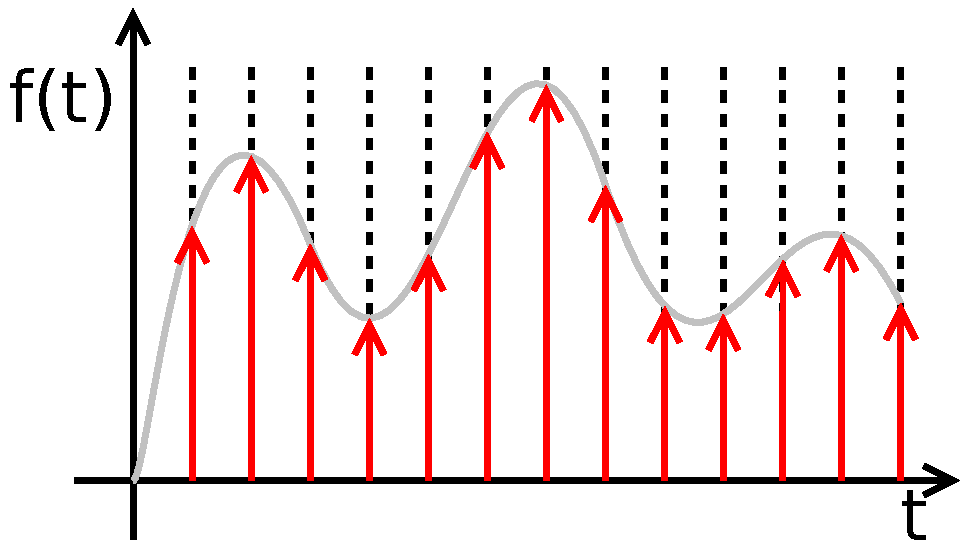
\includegraphics[width=.8\textwidth]{pic/sampled-1.pdf}
  \caption{Temporal quantisation of continuous 1-D signal.}
  \label{fig:sampled-1}  
\end{figure}

We know from \emph{Niquist-Shannon sampling theorem} that perfect
reconstruction of a signal is possible when the sampling frequency is
greater than twice the maximum frequency of the signal being sampled,
or equivalently, when the \emph{Nyquist frequency} (half the sample
rate) exceeds the highest frequency of the signal being
sampled. Because the hearing range in most human beings is 20 Hz--20
kHz, audio compact discs use a 44.1 kHz sampling rate. Other popular
rates in audio production are 48 kHz, 96 kHz and 192 kHz. Sampling
rates bellow 44.1 kHz are used also in old computer games that were
limited by the computing power and low bandwidth systems such as
telephone, where low cost and proper understanding of human speech is
more important than audio fidelity.

The sound representation mechanism itself does not vary with the
sampling rate, and thus supporting various rates depends more on the
implementation of the signal processing units and the overall
performance of the system, with the CPU being able to process so many
samples per second being the biggest constraint.

\subsubsection{Spatial quantisation}

\begin{figure}[h!]
  \centering
  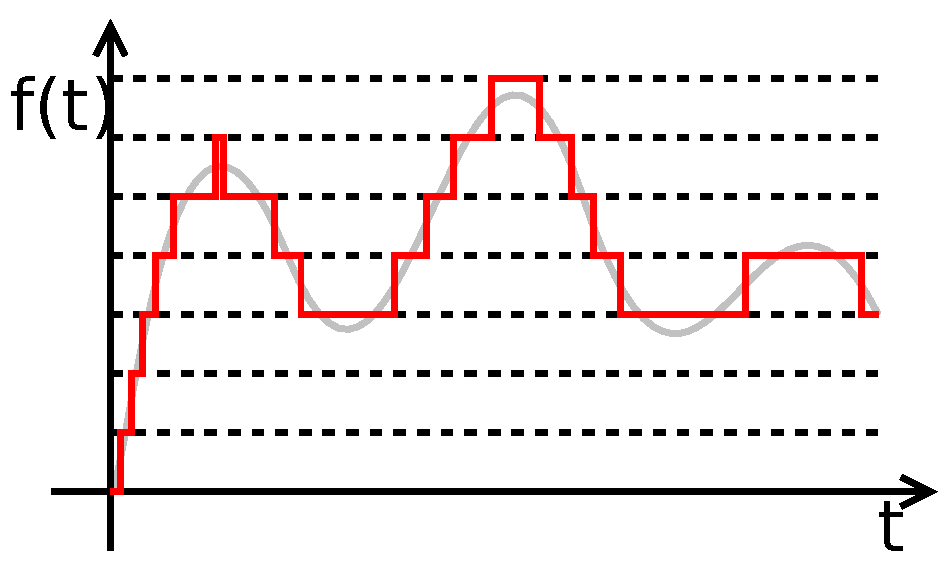
\includegraphics[width=.8\textwidth]{pic/sampled-2.pdf}
  \caption{Spatial quantisation of continuous 1-D signal.}
  \label{fig:sampled-2}  
\end{figure}

\begin{figure}[h!]
  \centering
  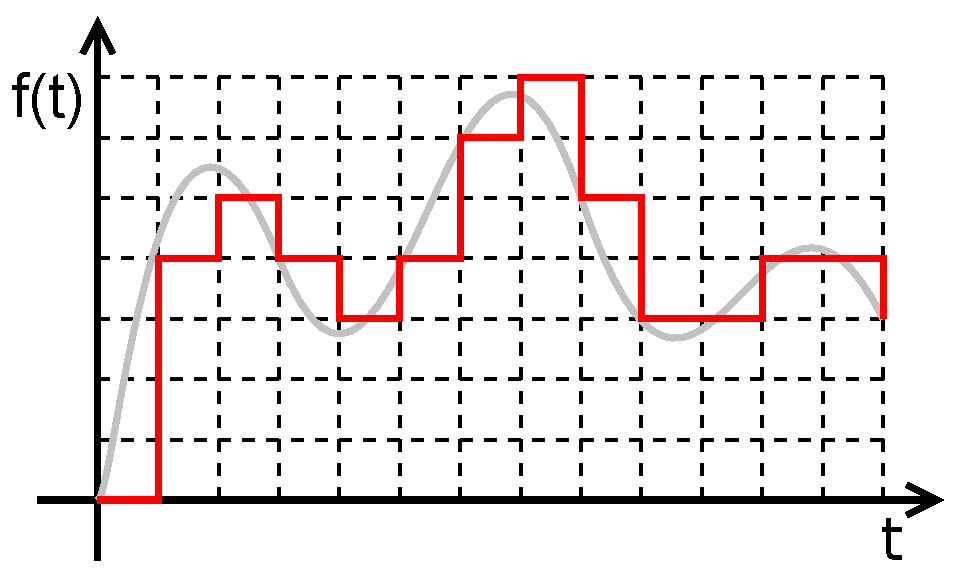
\includegraphics[width=.8\textwidth]{pic/sampled-3.pdf}
  \caption{Fully quantised continuous 1-D signal}
  \label{fig:sampled-3}
\end{figure}

Spatial quantisation determines how many possible values can a sample
take in our finite and discrete scale. Figure \ref{fig:sampled-2}
shows a linear spatial quantisation, represented by the dotted lines
parallel to the abscissa axis. That is a best fit quantisation
assuming a time continuum, in practise, spatial quantisation is
applied over an already discreet time, figure \ref{sampled-3} combines
the quantisations of figures \ref{fig:sampled-1} and
\ref{sampled-2}. In a computer system, spatial quantisation is mostly
determined by the size in bits of the underlying type used to store
the samples. Also, the quantisation is affected by how we space the
different plausible values. In practise, linear quantisation
---i.e. equally spaced samples--- is most in audio formats targeted at
music, but logarithmic and other non-linear divisions are common in
telephony and other lo-fi systems. Note that using floating point
values to represent samples, as it is often done in software
synthesis, provides an implicitly logarithmic audio quantisation. An
audio CD uses a \emph{bitdepth} of 16 bit with samples that can take
$65.536$ possible values while professional audio uses 24 bit or 32
bit samples. We can even see systems using 64 bit samples during the
processing to avoid accumulative rounding problems due to heavy
arithmetic. The \emph{dynamic range} of a signal with $Q$-bits
quantisation is:
\begin{equation}
  \mathrm{DR_{ADC}} = 20 \times \log_{10}(2^Q) = (6.02 \cdot Q)\, \mathrm{dB}
\end{equation}
The maximum \emph{signal-to-noise} ratio for such a system is:
\begin{equation}
  \mathrm{SNR_{ADC}} =  \left (1.76 + 6.02 \cdot Q \right )\ \mathrm{dB}
\end{equation}

Most analog systems are said to have a dynamic range of around 80 dB
\cite{fries05digital}. Digital audio CD have a theoretical
dynamic range of 96 db --- actual value is around 90 db due to
processing. Human hearing pain level is at 135 db but actually
prolonged exposure to such loud sound can cause damage. A loud rock
concert is around 120 dB and a classical music performance is at
110 db \cite{ludwig09music}, thus requiring bitdepth of at least 24
bit (theoretical dynamic range of 144 dB) for perfect fidelity.

There are some other aspects related to representation of samples in a
computer, such as the \emph{signedness} of the underlying type. Signed
types are usually considered more convenient for audio signals as 0
can be easily recognised as the still no-sound value simplifying
computations. Another important factor is whether we use \emph{fixed
  point} or \emph{floating point} arithmetic. While fixed point is
used in low-cost DSP hardware, floating point is the most common
representation in current audio software as nowadays processors are
optimised for SIMD\footnote{Single Instruction Multimple Data, as
  supported by MMX, 3D Now! and SSE extensions in Intel and AMD chips}
floating point arithmetic. Moreover, the algorithms implementation is
much harder to encode because products produce greater values and
there are many ways on how to account the carry.  Actually, even while
the actual bitdepth (the bit for the mantissa) of a 32 bit floating
point is the same of a 24 bit fixed point, then a 32 bit fixed point
will have a quite lower \emph{quantization error}, but the dynamic
range and SNR of a floating point is much higher because the
values are spaced logarithmically over a huge range
\cite{smith02dsp}. Another factor is the \emph{endianess} of fixed
point values but is relevant only when interfacing with file formats
and output devices.

\subsubsection{Channel space}

Because our hearing system is dicotomically symmetric, audio engineers
discovered that much better fidelity can be achieved by reproducing
the sound with some differences from two separate loudspeakers. This
is the well-known \emph{stereophonic} sound, commonly named just
\emph{stereo}. For representing such a signal, two different streams
of information are needed for the left and right channels. Moreover,
nowdays \emph{quadraphonic}, and \emph{surround} sound with varying
numbers of channels up to 20.2 are used in different systems.

We call \emph{channel space} to the set of semantic channels we use in
some sort of audio representation --- e.g. stereo audio has channel
space with $left$ and $right$ elements. We use the term
\emph{frame} to call a set of samples coincident in time, this is, the
samples of the various channels at a given time point. Thus, we will
use most of the time the more accurate term \emph{frame rate}.

\begin{figure}[h]
  \centering
  \subfloat[]{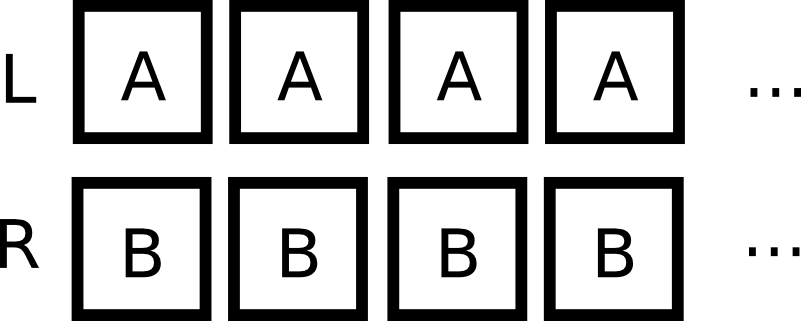
\includegraphics[width=2in]{pic/fmt-planar.png}}\;
  \subfloat[]{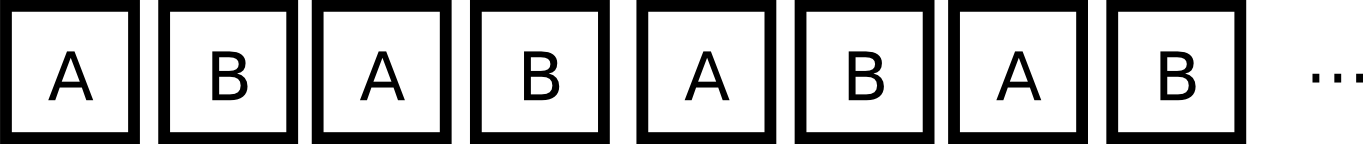
\includegraphics[width=3in]{pic/fmt-interleaved.png}}
  \caption{Multi-channal data in planar (a) and interleaved (b) form.}
  \label{fig:interleaving}
\end{figure}

This rises the problem on how to linearise the multi channel data. The
most common mechanism in domestic hardware is by \emph{interleaving}
the samples of different channels, this is, by storing the frames
sequentially. However, high-end hardware often accepts data in
non-interleaved form where the samples of each channel is stored in a
separate sequence. In this document, we borrow from the image
processing world the term \emph{planar} to refer to non-interleaved
data. Software doing a lot of processing of the audio signal often
chooses this representation as it is easier to scale to varying number
of channels and split the signal to do per-channel filtering. Figure
\ref{fig:interleaving} compares visually the interleaved and planar
formats.

Another issue is the order in which the data from different semantic
channels is stored. We call a \emph{channel layout} a bijection $L : C
\rightarrow \mathbb{Z}_{\|C\|}$, where $C$ is a given \emph{channel
  space}. For example, the mapping $\{ left
\mapsto 0, right \mapsto 1 \}$ is a common layout for stereo sound,
but $\{ left \mapsto 1, right \mapsto 0 \}$ is sometimes used too.

The last concern related to quantisation is
\emph{dithering}. Dithering is the process of adding a white noise
signal in a range similar to that of the quantisation step
---e.g. $[-2^{-n}, 2^{-n}]$ for a linear $n$-bit quantisation--- prior
to doing the quantisation itself. While this increases the overall
SNR, the perceived subjective distortion is much smaller as harmonics
introduced by the regularity of quantisation error are aliased; with a
proper noise model we can even push the harmonic artifacts outside the
audible range to achieve minor distortion \cite{vanderkooy87dither,
  lipshitz91minimally}.

\subsection{Common solutions}

As we have already noticed, 32 bit floating point sound with planar
left-right layout the most common in software of our kind during
internal processing. As most of this software is written in C, a
simple \texttt{float**} does the job. This was, actually, the internal
representation used in GNU Psychosynth in versions prior to 0.2.0,
wrapped in the \texttt{audio\_buffer} class.

However, this design starts to wobble whenever one has to interface
with some other library or hardware using a different format. Thus,
the \texttt{audio\_buffer} class provided different
\texttt{interleave\_*} and \texttt{deinterleave\_*}, where the
asterisk can be substituted by different sample formats like
\texttt{s16} or \texttt{s32} (fixed point signed 16 bit and 32 bit
respectively). This is very inconvenient because, as we have seen
through this section, many orthogonal factor affect audio
representation inducing a combinatorial explosion of format conversion
functions. Take a look at the 64 different read and write functions in
the \texttt{pcm.c} file of the
LibSndfile\footnote{\url{http://www.mega-nerd.com/libsndfile/}}
library.

This is a maintenance hell, but using the common means for abstracting
orthogonal behaviour variability, i.e. dynamic polymorphism, is simply
not an option in any audio software which supports real-time
operation.

\subsection{A generic approach: Boost.GIL}

However, there is a piece of software that proved that this issue can
be solved in C++ using static polymorphism. This is the Generic Image
Library\footnote{\url{http://stlab.adobe.com/gil}} which was developed
by Lubomir Bourdev et. Al inside Adobe Software Technology Lab that
was later include inside the Boost library distribution.

While sound and image manipulation are quite different, specially from
the psycho-perceptive point of view, they are both a signal processing
problem and thus share a lot in the representational issue. By
realising of a proper conceptual mapping between both worlds (table
\ref{tab:gilmap}), most of the library design and even quite a lot of
code of Boost.GIL can be reused to build a unique state-of-the-art
sound processing library that addresses the aforementioned issues in
an orthogonal generic manner while maintaining near-optimal
performance.

\begin{table}[h]
  \centering
  \begin{tabular}{c|c}
    Boost.GIL & Psynth.Sound \\ \hline\hline
    Channel   & Sample \\
    Color     & Channel \\
    Color Space & Channel Space \\
    Color Layout & Channel Layout \\
    Pixel & Frame \\
    View & Range \\
    Image & Buffer
  \end{tabular}
  \caption{Terminology map from \texttt{boost::gil} to \texttt{psynth::sound}}
  \label{tab:gilmap}
\end{table}

An \emph{image} is bidimensional matrix of \emph{pixels}, that capture
the properties of light electromagnetic waveform at those discrete
points. Each pixel, however, is decomposed in several \emph{colors}
that, for example, capture the intensity in the red, green and blue
sensors of a CCD camera. As there are different ways of decomposing an
audio frame (e.g, stereo, surround, etc.), there are different ways of
decomposing a pixel into several values, known as the \emph{color
  space} (e.g, RGB, CMYK, YUV, etc.). Boost.GIL uses the term
\emph{channel} to name the individual value of one those color
components.

In our audio framework, a \emph{buffer} is unidimensional array of
\emph{frames} that represent a sound or part of a sound --- sound is
continuous and thus we usually process it in chunks. The reader might
note that the the data in a buffer being arranged along the
\emph{time} dimension while the dimensions of an image represent
\emph{physical space} makes these entities completely different from
the processing point of view. However, they share most representation
problems, with sound representation being actually a sub-problem of
image representation, as we have one dimension less. The samples in a
series of audio frames can be stored in an interleaved or planar
fashion as happens with the channels of a pixel. Also, both channels
and samples can vary in signedness, fixed/floating point, bitdepth,
etc.

Those already familiar with Boost.GIL can thus already understand
easily our Psynth.Sound module design and implementation that we are
to describe in the following section.

\section{Design}

This section describes the design of the modules implemented in this
layer. We will first introduce some advanced techniques used in the
design that the reader might be unfamiliar with. Then, sections
\ref{sec:ns-sound-beg} to \ref{sec:ns-sound-end} will describe the
classes in the \texttt{psynth::sound} namespace, section
\ref{sec:ns-io} will be dedicated to the \texttt{psynth::io} namespace
and finally section \ref{sec:ns-synth} to the \texttt{psynth::synth}
namespace. \texttt{psynth::io} and \texttt{psynth::synth} are
independent from eachother and both depend on
\texttt{psynth::sound}. Still, from the architectural point of view
they are all considered to be on the same layer --- the ``synth''
layer dedicated to mostly statically arranged sound synthesis and
processing.

\subsection{Core techniques}

The Boost.GIL and thus the Psynth.Sound modules design makes heavy use
of static polymorphism and generic programming via C++ templates to
achieve generality without runtime overhead. We are going to introduce
advanced techniques used in generic programming for the reader
unfamiliar with this programming paradigm.

\subsubsection{Concepts}
\label{sec:concepts}.

\emph{Concepts} \cite{jarvi10concept} are to generic programming what
\emph{interfaces} --- pure abstract classes in C++ --- are to object
oriented programming: they specify the requirements on some
type. However there, are few substantial differences. (1) While
interfaces can only specify the method signatures of its instances, a
concept can specify most syntactic constraints on a type, like the
existence of free functions, operators, nested types, etc. (2) While
dispatching through interfaces requires, at least, a dereference,
addition and function call \cite{driesen96direct}, when using concepts
the concrete function to be executed can be determined and even
inlined at compile-time. (3) One can not declare that a type satisfies
an interface separately from the type definition, but one can say that
a type models a concept at any point of the program. (4) Thus, no
primitive type defines any virtual interface, but one can turn any
primitive type into an instance of any concept via a
\texttt{concept\_map}. (5) Actually, the syntactic properties defined
by a concept its models may differ, but they are matched via the
\texttt{concept\_map}. In fact, C++ concepts are more similar to
Haskell \emph{type classes}, with \texttt{instace} doing the job of
\texttt{concept\_map} \cite{bernardy08comparison}.

Concepts are an extension to the template mechanism to add type
checking for it. In fact, checking and dispatching on requirements can
be achieved with techniques like SFINAE (Substitution Failure Is Not
an Error) \cite{vandervoorde08templates}. Property (5) of our concepts
can be simulated with \emph{traits} \cite{c++traits}. However, both
compiler errors and the code using templates without concepts is
usually much more unreadable.

The proposal of adding concepts to the C++ language was rejected last
year by the standardisation committee and thus we can not use them in
our code. However, Boost.GIL is very influeced by Alexander Stepanov's
deductive approach to computer programming using generic programming
and modeling with concepts, that he elegantly describes in his
master-piece ``Elements of Programming''
\cite{stepanov09elements}. Actually Stepanov worked several years in
Adobe where he held a course ``Foundations of Programming'' based on
his book. Thus, the \emph{modeling} of the library extensively uses
concepts. Its implementation uses a limited form of concept checking
via the Boost.ConceptCheck\footnote{
  Boost.ConceptCheck: \url{http://www.boost.org/doc/libs/release/libs/concept_check/concept_check.htm}}
\cite{siek00concept} library, however, enabling this library in
release mode can affect performance and its syntax is quite more
cumbersome than the concepts in the C++ standard proposal. For
consistency with the Boost.GIL documentation we will use the concept
syntax proposed in the proposal N2081 to the standardisation committee
\cite{gregor06concept}.

The following example defines a concept that is satisfied by every
type that has an \texttt{operator<}:

\begin{lstlisting}
concept LessThanComparable<typename T> {
  bool operator< (T, T);
};
\end{lstlisting}

This allows us to write a generic function that depends on the
existence of a less-than comparator for the parametrised type:

\begin{lstlisting}
template<LessThanComparable T>
const T& min (const T& x, const T& y) {
  return x < y? x : y;
}
\end{lstlisting}

An alternative syntax for specifying that \texttt{T} must satisify the
\texttt{LessThanComparable} concept is the \texttt{where} clause:

\begin{lstlisting}
template<typename T>
    where LessThanComparable<T>
const T& min (const T& x, const T& y) ...
\end{lstlisting}

In fact, this is the only valid syntax when the concept affects
multiple types. Also, the \texttt{where} clause can be used inside
concept definitions to provide specialisation.

Specifying that a type models a concept is done with the
\texttt{concept\_map} device. If the type naturally models the
concept, we can just use:

\begin{lstlisting}
concept_map LessThanComparable<int> {}
\end{lstlisting}

Note that these trivial concept mappings can be avoided by using the
\texttt{auto} keyword in front of the \texttt{concept} keyword in the
concept definition. However, it might happen that a type requires some
wrapping to satisfy the concept. We can do this in the concept map
definition itself.

\begin{lstlisting}
concept_map LessThanComparable<char*> {
  bool operator< (char* a, char* b) {
    return strcmp (a, b) < 0;
  }
}
\end{lstlisting}

Note that this last piece of code is an example of a bad usage of
concept maps, as this specialises the mapping for pointers changing
the expected semantics.

This should suffice as an introduction to concepts in order to
understand the concept definitions that we will later show when
modelling our system. A more detailed view can be read in the cited
bibliography, with \cite{jarvi10concept} being the most updated and
useful from a programmer point of view.

\subsubsection{Metaprogramming}

The C++ template system is Turing complete
\cite{veldhuizen03templates}, thus it can be used to perform any
computation at \emph{compile time}. This was first noted in 1994 by
Erwin Unruh who, in the middle of a C++ standardisation committee,
wrote a template meta-program that outputted the first $N$ prime
numbers on the console using compiler errors \cite{unruh94prime}. Even
though this might seem just a crazy puzzle game, it can be used in
practise and actually new Boost libraries use it extensively. A very
gentle introduction to template metaprogramming can be found in
\cite{alexandrescu01modern}, where Alexandrescu uses them to
instantiate design patterns as generic C++ libraries. A deeper
reference is Abraham's \cite{abrahams04meta}, which focuses on the
Boost Metaprogramming Library\footnote{The Boost.MPL:
  www.boost.org/doc/libs/release/libs/mpl} and introduces the usage of
metaprogramming for building Embedded Domain Specific Languages (EDSL)
in C++. This Boost.MPL, providing reusable meta data structures and
algorithms, is the de-facto standard library for template
metaprogramming\footnote{It is often called ``the STL of template
  metaprogramming''.} and we will use it in our implementation.

Template metaprogramming is possible thanks to \emph{partial template
  specialisation}, that allows giving an alternate definition for a
pattern matched subset of its possible parameter values. A
\emph{metafunction} is thus just a template \texttt{class} or
\texttt{struct} with a public member that holds the result of the
function. It is up to the programmer to choose the naming convention
for the result members of the metafunctions, in the following, we will
use Abraham's style calling \texttt{type} for result values that are a
type, and \texttt{value} for integral values. Listing \ref{lst:fib}
illustrates how can we write and use a metafunction for computing the
$n$-th Fibonacci number.

\begin{lstlisting}[float=h!, 
  caption=Metaprogram for computing the Nth Fibonacci number,
  label=lst:fib]
template <int N>
struct fib {
  enum { 
    value = fib<N-1>::value + fib<N-2>::value; 
  };
};

template <>
struct fib <0> {
  enum { value = 0 };
};

template <>
struct fib <1> {
  enum { value = 1 };
};

int main () {
  return fib<42>::value;
}  
\end{lstlisting}

The program returns the forty-second Fibonacci value. However, it will
take no time to execute, because the number is computed at compile
time. We use recursion to define the metafunction for the general case
and the specialise for the base cases.

If we consider the template system as a meta-language on its own, we
should describe its most outstanding semantic properties. It is a pure
functional programming language, because variables are immutable. It
is lexically scoped. It supports both lazy and strict evaluation,
depending on whether we choose to access the nested \texttt{type}
result name at call site or value usage type. When we look at the meta
type system, we find three meta types: types (which are duck-typed
records), integrals (e.g. \texttt{int}, \texttt{char}, \texttt{bool}
...) and meta-functions (i.e. templates).

The fact that records are duck typed but integrals and metafunctions
cause several inconveniences in practice, specially when dealing with
the later. For example, in the absence of template aliases, returning
a metafunction produced by another function requires defining a nested
struct that inherits from the actual synthesised value. Also, the
template signature should be specified on a template parameter
expecting a template.

In order to simplify our meta type system we shall wrap constants in a
type like on listing \ref{lst:integral_c}.

\begin{lstlisting}[float, 
  caption=Integral constant nullary metafunction  wrapper.,
  label=lst:integral_c]
template <typename T, T V>
struct integral_c
{
  BOOST_STATIC_CONSTANT(T, value = V);
  typedef integral_c<T, V> type;
};
\end{lstlisting}

There are a couple of issues regarding this definition worth
explaining. First, the \texttt{BOOST\_STATIC\_CONSTANT} macro is used
to define a constant. Internally, it will try to use \texttt{enum} or
any other mechanism available to actually define the constant such
that the compiler is not tempted to allocate static memory for the
constant. Second, the \texttt{typedef} referring to itself turns a
constant value into a self returning nullary meta-function. This can
be very convenient because, for example, it allows using
\emph{value}\texttt{::type::value} always on the value usage point,
allowing the caller or producer of the value to choose whether he
wants to evaluate the value lazily.

Because we just wrapped values into a type, we can simplify our
conventional definition of \emph{metafunction}: a meta-function is any
type --- template or not --- that has a nested type called
\texttt{type}.

Now we should also turn metafunctions into first class entities of the
meta-language. We just add a new level of indirection and define a
\emph{metafunction class} as a type with a nested template
metafunction called \texttt{apply}. The example in listing
\ref{lst:high_order_fib} also illustrates the metafunction forwarding
technique when defining the nested \texttt{apply} metafunction by
inheriting from \texttt{fib}.

\begin{lstlisting}[float, caption=Metafunction class for
  computing Fibonacci numbers. We suppose that the previous
  \texttt{fib} definition uses \texttt{integral\_c} to wrap its
  parameters and return types., label=lst:high_order_fib]
struct fib_class { 
   template <class N>
   struct apply : public fib<N> {};
};

int main ()
{
  return fib_class::apply<integral_c<int, 42>>::type::value;
}
\end{lstlisting}

Using this convention the MPL library defines many useful high order
metafunctions that take metafunction classes as input, like
\texttt{mpl::fold} and \texttt{mpl::transform}. Note that it is not
needed to define metafunction classes for all our metafunctions,
instead, we shall convert them when needed using the
\texttt{mpl::quote}\emph{N} functions and the \texttt{mpl::lambda}
facility.

\subsection{Core concepts}
\label{sec:ns-sound-beg}
We are now ready to understand the main design and implementation
techniques used in our generic library. Because the library is
\emph{generic}, in the sense of generic programming, most algorithms
and data structures are parametrised such that they can be
instantiated with any concrete type modelling some concepts as we
suggested in section \ref{sec:concepts}. Thus, traditional modelling
techniques like the Unified Modelling Language are not useful since
they are intended for object oriented design.

We are going to follow the following methodology for describing the
library. First, we will name a concept and give a brief description of
its purpose. Then, we will define the concept using the notation
described in section \ref{sec:concepts} and finally we will enumerate
and describe some models for such concept.

For brevity, we will omit basic concepts such as
\texttt{Copy\-Constructible}, \texttt{Regular}, \texttt{Metafunction},
etc. Their complete definition should be evident and an interested
reader can find most of them in \cite{stepanov09elements}.

\subsubsection{{ChannelSpaceConcept}}

A channel space is a MPL sequence (like \type{mpl::list}) of whose
elements channel tags (empty types giving a name for the semantic
channel).

\begin{lstlisting}
concept ChannelSpaceConcept<MPLRandomAccessSequence Cs> 
{};
\end{lstlisting}

Some example models include \texttt{stereo\-\_space} or
\texttt{surround\-\_space}. An example on how a user of the library can
define his own channel space follows.

\begin{lstlisting}
struct left_channel {};
struct right_channel {};

typedef mpl::vector<left_channel, right_channel> stereo_space;
\end{lstlisting}

A related trivial concept is
\texttt{Channel\-Space\-Compatible\-Con\-cept}. Two channel spaces are
compatible if they are the same. In fact, this leaks the underlying
MPL sequence type used in the channel space through the abstraction,
because spaces with the same set of semantic channels might be found
incompatible, but it suffices in practise.

\subsubsection{{SampleMappingConcept}}

An MPL Random Access Sequence, whose elements model
\texttt{MPLIntegralConstant} (like \texttt{mpl::int\_}) representing a
permutation of the channels in the channel space, thus specifying the
layout.

\begin{lstlisting}
concept SampleMappingConcept<MPLRandomAccessSequence CM> {
};
\end{lstlisting}

The \emph{layout} of a frame based type is a channel space plus a
sample mapping, as defined by:

\begin{lstlisting}
template <typename ChannelSpace,
	  typename SampleMapping = boost::mpl::range_c<
	      int, 0, boost::mpl::size<ChannelSpace>::value> >
struct layout
{
    typedef ChannelSpace   channel_space;
    typedef SampleMapping  sample_mapping;
};
\end{lstlisting}

The sample mapping is usually directly defined in the layout, if
needed at all --- the default sample mapping is the normal order in
the channel space. For example, the reversed stereo layout is defined
as:

\begin{lstlisting}
typedef layout<stereo_space, mpl::vector2_c<int, 1, 0>> rlstereo_layout;
\end{lstlisting}

\subsubsection{{SampleConcept}}

A \emph{sample} is the type we use to represent the amplitude of a
channel at certain point in time.

\begin{lstlisting}
concept SampleConcept<typename T> :
             EqualityComparable<T> {
    typename value_type      = T;
    // use sample_traits<T>::value_type to access it
    typename reference       = T&;
    // use sample_traits<T>::reference to access it
    typename pointer         = T*;
    // use sample_traits<T>::pointer to access it
    typename const_reference = const T&;
    // use sample_traits<T>::const_reference to access it
    typename const_pointer   = const T*;
    // use sample_traits<T>::const_pointer to access it
    static const bool is_mutable;
    // use sample_traits<T>::is_mutable to access it

    static T min_value(); 
    // use sample_traits<T>::min_value to access it
    static T zero_value(); 
    // use sample_traits<T>::zero_value to access it
    static T max_value(); 
    // use sample_traits<T>::min_value to access it
};
\end{lstlisting}

Built-in scalar types like \texttt{char}, \texttt{int} or
\texttt{float} model \texttt{Sample\-Concept} by default. 

The \texttt{scoped\_sample\_value<Type, Min, Max, Zero>} template
class models the concept whenever \texttt{Type} is a scalar type and
\texttt{Min}, \texttt{Zero} and \texttt{Max} satisfy:
\begin{equation}
Min < Zero < Max \land \forall x \in Type, x + Zero = x
\end{equation}
Note that, in order to avoid the limitation of floating point values
not being usable as template arguments, \texttt{Min}, \texttt{Zero}
and \texttt{Max} should be a type with a static method
\texttt{apply()} that returns the actual value. It should be used to
constraint the ``clipping thresholds'' of floating point types. For
example, the \texttt{bits32sf} model defined as:

\begin{lstlisting}
typedef scoped_sample<float,
                      float_minus_one,
                      float_zero,
                      float_one> bits32sf;
\end{lstlisting}

User defined types should specialise \texttt{sample\-\_traits} to map
the concept.

Related trivial concepts are \texttt{MutableSampleConcept} and
\texttt{SampleValueConcept} (a sample that is also \texttt{Regular}).

\subsubsection{{SampleConvertibleConcept}}

Because casting does not suffice in most cases, one should
override a \texttt{T sample\_convert (U)} function for \texttt{U} to
be convertible into \texttt{T}.

\begin{lstlisting}
concept SampleConvertibleConcept<SampleConcept SrcSample,
     SampleValueConcept DstSample> {
    DstSample sample_convert (const SrcSample&);
};
\end{lstlisting}

The library provides overrides for \texttt{sample\_convert} making
most supplied sample types being convertible too.

\subsubsection{{ChannelBaseConcept}}

A \emph{channel base} is a container of channel elements (such as
samples, sample references or sample pointers).

The most common use of channel base is in the implementation of a
frame, in which case the channel elements are sample values. The
channel base concept, however, can be used in other scenarios. For
example, a planar frame has samples that are not contiguous in
memory. Its reference is a proxy class that uses a channel base whose
elements are sample references. Its iterator uses a channel base whose
elements are sample iterators.

\begin{lstlisting}
concept ChannelBaseConcept<typename T> :
      CopyConstructible<T>, EqualityComparable<T>
{
    // a Psynth layout (the channel space and element permutation)
    typename layout;     
        
    // The type of K-th element
    template <int K> struct kth_element_type;
    where Metafunction<kth_element_type>;
    
    // The result of at_c
    template <int K> 
    struct kth_element_const_reference_type;
    where Metafunction<
            kth_element_const_reference_type>;        
    
    template <int K> 
    kth_element_const_reference_type<T,K>::type at_c(T);

    // Copy-constructible and equality comparable 
    // with other compatible channel bases
    template <ChannelBaseConcept T2> 
        where { ChannelBasesCompatibleConcept<T,T2> } 
        T::T(T2);
    template <ChannelBaseConcept T2> 
        where { ChannelBasesCompatibleConcept<T,T2> } 
        bool operator==(const T&, const T2&);
    template <ChannelBaseConcept T2> 
        where { ChannelBasesCompatibleConcept<T,T2> } 
        bool operator!=(const T&, const T2&);
};
\end{lstlisting}

A channel base must have an associated layout (which consists of a
channel space, as well as an ordering of the samples).  There are two
ways to index the elements of a channel base: A physical index
corresponds to the way they are ordered in memory, and a semantic
index corresponds to the way the elements are ordered in their channel
space.  For example, in the stereo channel space the elements are
ordered as \texttt{\{left\_channel, right\_channel\}}. For a channel
base with a RL-stereo layout, the first element in physical ordering
is the right element, whereas the first semantic element is the left
one.  Models of \texttt{ChannelBaseConcept} are required to provide
the \texttt{at\_c<K>(ChannelBase)} function, which allows for
accessing the elements based on their physical order. Psynth provides
a \texttt{semantic\_at\_c<K>(ChannelBase)} function (described
later) which can operate on any model of \texttt{ChannelBaseConcept}
and returns the corresponding semantic element.

A related concept is \texttt{Mutable\-Channel\-Base\-Con\-cept} and
\texttt{Chan\-nel\-Base\-Value\-Con\-cept} with the excepted
definition. There is also the concept
\type{Channel\-Bases\-Compatible\-Concept}. Two channel bases are
compatible if they have the same channel space and their elements are
compatible, semantic-pairwise.

\subsubsection{{HomogeneousChannelBaseConcept}}

Channel base whose elements all have the same type.

\begin{lstlisting}
concept HomogeneousChannelBaseConcept<
            ChannelBaseConcept CB> 
{
    // For all K in [0 ... size<C1>::value-1):
    //     where SameType<kth_element_type<CB,K>::type,
    //                    kth_element_type<CB,K+1>::type>;    
    kth_element_const_reference_type<CB,0>::type dynamic_at_c(
           const CB&, std::size_t n) const;
};  
\end{lstlisting}

Related concepts \type{MutableHomogeneousChannel\-Base\-Con\-cept} and
\type{Ho\-mo\-geneous\-ChannelBaseValueConcept} have the expected
definition.

The library provides an \texttt{homogeneous\_channel\_base} class that
models the concept.

\subsubsection{{FrameBasedConcept}}

Concept for all frame based constructs, such as frames themselves,
iterators, ranges and buffers whose value type is a frame. A
\texttt{FrameBased} type povides some metafunctions for accessing the
underlying channel space, sample mapping and whether the frame
representation is planar or interleaved.
  
\begin{lstlisting}
concept FrameBasedConcept<typename T> {
    typename channel_space_type<T>;     
        where Metafunction<channel_space_type<T> >;
        where ChannelSpaceConcept<channel_space_type<T>::type>;
    typename sample_mapping_type<T>; 
        where Metafunction<sample_mapping_type<T> >;  
        where SampleMappingConcept<sample_mapping_type<T>::type>;
    typename is_planar<T>;
        where Metafunction<is_planar<T> >;
        where SameType<is_planar<T>::type, bool>;
};  
\end{lstlisting}

There are many models for this in the library, like \type{buffer},
\type{buffer\_range}, \type{frame}, \type{bitaligned\_frame\_iterator},\\
\type{bitaligned\_frame\_reference}, \type{packed\_frame} and so on.

\subsubsection{{HomogeneousFrameBasedConcept}}

Concept for homogeneous frame-based constructs --- frame based with
the same sample type for all its channels. These should allow access
to the underlying sample type.

\begin{lstlisting}
concept HomogeneousFrameBasedConcept<FrameBasedConcept T> {
    typename sample_type<T>;         
        where Metafunction<sample_type<T> >;
        where SampleConcept<sample_type<T>::type>;
};
\end{lstlisting}

Most container and alike constructs in the library --- iteators,
buffers, ranges --- model this whenever the underlying frame is
homogeneous.

\subsubsection{{FrameConcept}}

A set of samples coincident in time, one per channel in the given
channel space.

\begin{lstlisting}
concept FrameConcept<typename F> :
            ChannelBaseConcept<F>, FrameBasedConcept<F> {    
    where is_frame<F>::type::value==true;
    // where for each K [0..size<F>::value-1]:
    //      SampleConcept<kth_element_type<F,K> >;
        
    typename F::value_type;       
        where FrameValueConcept<value_type>;
    typename F::reference;
        where FrameConcept<reference>;
    typename F::const_reference;  
        where FrameConcept<const_reference>;
    static const bool F::is_mutable;

    template <FrameConcept F2> where { FrameConcept<F,F2> } 
        F::F(F2);
    template <FrameConcept F2> where { FrameConcept<F,F2> } 
        bool operator==(const F&, const F2&);
    template <FrameConcept F2> where { FrameConcept<F,F2> } 
        bool operator!=(const F&, const F2&);
}; 
\end{lstlisting}

Related concepts are \type{MutableFrame\-Concept} and
\type{Frame\-Value\-Concept}, defined as usually.

Frame compatibility should be tested with the
\texttt{Frames\-Compatible\-Concept}.  Frames are compatible if their
samples and channel space types are compatible. Compatible frames can
be assigned and copy constructed from one another.


Provided models include \type{frame}, \type{packed\-\_frame},
\type{planar\-\_frame\-\_reference} and
\type{bit\-\_aligned\-\_frame\-\_reference}.

\subsubsection{{HomogeneousFrameConcept}}

A frame with all samples of the same type should also provide an
indexed access operator.

\begin{lstlisting}
concept HomogeneousFrameConcept<FrameConcept P> :
            HomogeneousChannelBaseConcept<P>, 
            HomogeneousFrameBasedConcept<P> 
{ 
     P::template element_const_reference_type<P>::type 
     operator[] (P p, std::size_t i) const 
     { return dynamic_at_c(p,i); }
};
\end{lstlisting}

Related concepts are \type{MutableHomogeneousFrameConcept} and
\type{HomogeneousFrameValueConcept}, defined as usually.

Provided models include \type{planar\_frame\_reference} and
\type{frame}.

\subsubsection{{FrameConvertibleConcept}}

A frame type is convertible to another frame type if there exist a
\texttt{channel\_convert} overload. Convertibility is non-symmetric
and implies that one frame can be converted to another, approximating
the value. Conversion is explicit and sometimes lossy.

\begin{lstlisting}
template <FrameConcept SrcFrame, MutableFrameConcept DstFrame>
concept FrameConvertibleConcept {
    void channel_convert(const SrcFrame&, DstFrame&);
};
\end{lstlisting}

Frame types provided by the library are convertible.

\subsubsection{{FrameDereferenceAdaptorConcept}}

Represents a unary function object that can be invoked upon
dereferencing a frame iterator. This can perform an arbitrary
computation, such as channel conversion or table lookup.

\begin{lstlisting}
concept FrameDereferenceAdaptorConcept<
             boost::UnaryFunctionConcept D>
        : DefaultConstructibleConcept<D>
        , base::CopyConstructibleConcept<D>
        , AssignableConcept<D>  
{
    typename const_type;
        where FrameDereferenceAdaptorConcept<const_t>;
    typename value_type;
        where FrameValueConcept<value_type>;
    typename reference;         // may be mutable
    typename const_reference;   // must not be mutable
    static const bool D::is_mutable;

    where Convertible<value_type,result_type>;
};
\end{lstlisting}

The \type{channel\_convert\_deref\_fn} provides a model that performs
channel conversion.

\subsubsection{{FrameIteratorConcept}}

An STL random access traversal iterator over a model of
\type{FrameConcept}. Our iterators must provide some extra
metafunctions.

\begin{lstlisting}
concept FrameIteratorConcept<typename Iterator> 
        : boost_concepts::RandomAccessTraversalConcept<Iterator>
        , FrameBasedConcept<Iterator> 
{
    where FrameValueConcept<value_type>;
    typename const_iterator_type<It>::type;         
        where FrameIteratorConcept<const_iterator_type<It>::type>;
    static const bool  iterator_is_mutable<It>::type::value;          
    static const bool  is_iterator_adaptor<It>::type::value;
    // is it an iterator adaptor
};
\end{lstlisting}

Related concepts include \type{MutableFrame\-Iterator\-Concept},
defined as usually. The related \texttt{Has\-Dynamic\-StepTypeConcept}
is modelled by those iterator types with an overload for the
\type{dynamic\-\_step\-\_type} metafunction returning a similar
iterator that models \texttt{Step\-Iterator\-Concept}.

Models include \type{T*} where \type{T} is a frame or
\type{bitaligned\-\_frame\-\_iterator},
\texttt{memory\-\_based\-\_step\-\_iterator} and
\type{planar\-\_frame\-\_iterator}.

\subsubsection{{MemoryBasedIteratorConcept}}

Iterator that advances by a specified step. Concept of a random-access
iterator that can be advanced in memory units (bytes or bits).

\begin{lstlisting}
concept MemoryBasedIteratorConcept<
          boost_concepts::RandomAccessTraversalConcept Iterator> 
{
    typename byte_to_memunit<Iterator>;
    where metafunction<byte_to_memunit<Iterator> >;
    std::ptrdiff_t memunit_step(const Iterator&);
    std::ptrdiff_t memunit_distance(const Iterator& , const Iterator&);
    void memunit_advance(Iterator&, std::ptrdiff_t diff);
    Iterator memunit_advanced(const Iterator& p,
    std::ptrdiff_t diff)
    { Iterator tmp; memunit_advance(tmp,diff); return tmp; }
    Iterator::reference memunit_advanced_ref(
    const Iterator& p, std::ptrdiff_t diff) 
    { return *memunit_advanced(p,diff); }
};
\end{lstlisting}

Iterators defined by our library are memory based.

\subsubsection{StepIteratorConcept}

Step iterators are iterators that have can be set a step that skips
elements.

\begin{lstlisting}
concept StepIteratorConcept<
        boost_concepts::ForwardTraversalConcept Iterator> {
    template <Integral D> void Iterator::set_step(D step);
};
\end{lstlisting}

A related \type{MutableStepIteratorConcept} is defined as expected.
The class \type{memory\_based\_step\_iterator} models the concept.

\subsubsection{FrameIteratorConceptIteratorAdaptorConcept}

Iterator adaptor is a forward iterator adapting another forward
iterator.

\begin{lstlisting}
concept IteratorAdaptorConcept<
            boost_concepts::ForwardTraversalConcept Iterator> 
{
    where SameType<is_iterator_adaptor<Iterator>::type, 
                   boost::mpl::true_>;

    typename iterator_adaptor_get_base<Iterator>;
        where Metafunction<iterator_adaptor_get_base<Iterator> >;
        where boost_concepts::ForwardTraversalConcept<
                  iterator_adaptor_get_base<Iterator>::type>;
    
    typename another_iterator; 
    typename iterator_adaptor_rebind<Iterator,another_iterator>::type;
        where boost_concepts::ForwardTraversalConcept<another_iterator>;
        where IteratorAdaptorConcept<iterator_adaptor_rebind<
                 Iterator,another_iterator>::type>;

    const iterator_adaptor_get_base<Iterator>::type&
    Iterator::base() const;
};
\end{lstlisting}

There exist a related \type{MutableIteratorAdaptor\-Con\-cept} with the
usual definition. Classes \type{dereference\-\_iterator\-\_adaptor} and
\type{memory\-\_based\-\_step\-\_iterator} do model the concept.

\subsubsection{RandomAccessBufferRangeConcept}

This is a range, similar to the new STL range defined in C++0x, but
with some extra members for random access.

\begin{lstlisting}
concept RandomAccessBufferRangeConcept<base::Regular Range> 
{
    typename value_type;
    typename reference;       // result of dereferencing
    typename difference_type;
    // result of operator-(iterator,iterator)
    typename const_type; 
        where RandomAccessBufferRangeConcept<Range>;
    // same as Range, but over immutable values
    typename iterator; 
        where RandomAccessTraversalConcept<iterator>;
    // iterator over all values
    typename reverse_iterator;
        where RandomAccessTraversalConcept<reverse_iterator>; 
    typename size_type;       // the return value of size()

    // Defines the type of a range similar to this type, except it
    // invokes Deref upon dereferencing
    template <FrameDereferenceAdaptorConcept Deref>
    struct add_deref {
        typename type;
        where RandomAccessBufferRangeConcept<type>;
        static type make(const Range& v, const Deref& deref);
    };
    
    Range::Range(const iterator&, const size_type&);
    
    // total number of elements
    size_type        Range::size()       const; 
    reference        operator[](Range, const difference_type&) const;
    
    iterator         Range::begin()      const;
    iterator         Range::end()        const;
    reverse_iterator Range::rbegin()     const;
    reverse_iterator Range::rend()       const;
    iterator         Range::at(const size_type&);
};
\end{lstlisting}

There exists a \type{MutableRandomAccessBufferRange} with the usual
semantics.

\subsubsection{BufferRangeConcept}

A random access range over frames, it has extra information to get the
number of channels of the underlying frame type.

\begin{lstlisting}
concept BufferRangeConcept<RandomAccessBufferRangeConcept Range> 
{
    where FrameValueConcept<value_type>;
    std::size_t Range::num_channels() const;
};
\end{lstlisting}

There exists a related \type{MutableBufferRangeConcept} with the
expected definition. Also, there is a
\type{RangesAre\-Compati\-ble\-Concept}. Ranges are compatible if they have
the same channel spaces and compatible sample values. Constness and
layout are not important for compatibility.

The library provides the
\texttt{buffer\_range<Iterator>} model. There exists also a whole
family of \emph{range factories} that build a range or transform one
kind of range into another. These allow to build a buffer range on
top of raw data provided by an external library, lazily converting
from once frame type to another, obtaining sub parts of a frame, etc.

\subsubsection{RandomAccessBufferConcept}

A container of values. The values are accessible via an associated
range. Buffers are not ranges by themselves, because that generates
boilerplate due to constness problems --- a \type{const} range may
give mutable access to its frames, but a \type{const} buffer does
not, thus an algorithm that may mutate the frames but not the range
would have to provide two overloads.

\begin{lstlisting}
concept RandomAccessBufferConcept<typename Buf> : 
            base::Regular<Buf> {
    typename range; 
        where MutableRandomAccessBufferRangeConcept<range>;
    typename const_range = range::const_type;
    typename value_type  = range::value_type;
    typename allocator_type;

    Buf::Buf(point_t dims, std::size_t alignment=1);
    Buf::Buf(point_t dims, value_type fill_value, std::size_t alignment);
    
    void Buf::recreate(point_t new_dims, std::size_t alignment=1);
    void Buf::recreate(point_t new_dims, value_type fill_value,
                       std::size_t alignment);
    
    const const_range&   const_range(const Buf&);
    const range&         range(Buf&);
};
\end{lstlisting}

\subsubsection{BufferConcept}

A buffer containing frames.

\begin{lstlisting}
concept BufferConcept<RandomAccessBufferConcept Buf> {
    where MutableBufferRangeConcept<Buf::range>;
};
\end{lstlisting}

The \type{buffer} class models the concept.

\subsubsection{RandomAccessRingBufferRangeConcept}

Circular or ring buffers provide a virtual continuous flow of data
where one can write at one end and read from the other. There ring
buffer has a fixed size and the amount of available data plus free
space in the structure remains constant during operation, as seen in
figure \ref{fig:ringbuf}. This data structure is specially important
for passing audio data through different threads.

\begin{figure}[h!]
  \centering
  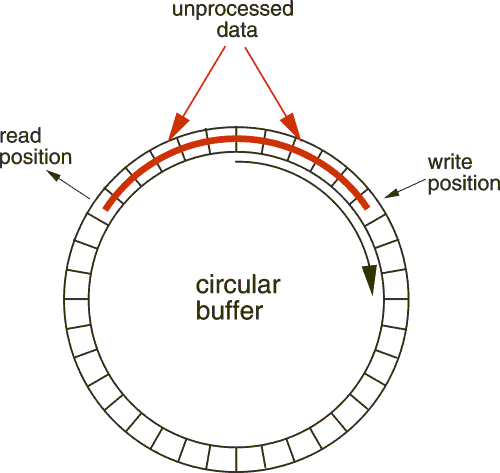
\includegraphics[width=.6\textwidth]{pic/ringbuffer.png}
  \caption{Ring buffer operation.}
  \label{fig:ringbuf}
\end{figure}

Our ring buffers wrap and underlying buffer range. Note that each ring
buffer range keeps its own write pointer, so using multiple ring
buffer ranges on the same data might lead to subtle problems.

\todo{A este concepto le faltan restricciones}.

\begin{lstlisting}
concept RandomAccessRingBufferRangeConcept<Regular R> 
{
    typedef range; where RandomAccessBufferRange<range>;

    typename reference = range::reference;
    typename size_type = range::size_type;
    typename value_type = range::size_type;
    typename difference_type = range::difference_type;
    
    typename unsafe_position;
    typename position;

    typename unsafe_iterator;
    typename iterator;
    
    R (const range& range);
    R& R::operator= (const range& r);

    size_type R::size () const;
    unsafe_iterator begin_unsafe () const;
    unsafe_iterator end_unsafe () const;
    iterator begin () const;
    iterator end () const;
    reference operator [] (difference_type i) const;    
    iterator at (difference_type i) const;
    unsafe_iterator unsafe_at (difference_type i) const;
    
    unsafe_position R::begin_unsafe_pos () const;
    unsafe_position R::end_unsafe_pos () const;
    position R::begin_pos () const;
    position R::end_pos () const;
    
    size_type R::available (const position& r) const;
    size_type R::available (const unsafe_position& r) const;    
    size_type R::available () const;
    ring_buffer_error R::check_position (const position& reader) const;

    template <class Position> range
    R::sub_range_one (const Position& p, size_type slice) const;
    template <class Position> range
    R::sub_range_two (const Position& p, size_type slice) const;
    
    template<class Position, class Range2>
    size_t R::read (Position& r, const Range2& range) const;
    template<class Position, class Range2, 
             class CC = default_channel_converter>
    size_t R::read_and_convert (Position& r, const Range2& range, 
                                CC cc = CC ()) const;
   
    template <class Range2>
    void R::write (const Range2& range);
    template <class Range2, class CC = default_channel_converter>
    void write_and_convert (const Range2& range, CC cc = CC ());

    bool is_backwards () const;
    void set_backwards ();
    
    // Total of data ever writen to the buffer.
    difference_type count () const;

    // Fix iterators after using set_backwards.
    position sync (const position& r) const;
};
\end{lstlisting}

There are some things worth mentioning about this concept. It supports
two different ways of manipulation. The STL alike iterator based
interface is provided for compatibility, but one should try to avoid
it for performance issues --- it has to check for having to wrap
around the end of the buffer on every iterator increment. Instead,
data should be added in chunks as large as possible with the
\emph{position} based interface --- the \type{read*} and \type{write*}
functions. When this is not possible, sometimes the
\type{sub\_range\_*} functions can provide a solution, allowing to
obtain the slices of the underlying range that represent a sub range
of the ring buffer.

\todo{Tal vez podrían desacoplarse las dos formas de manipular en dos
  conceptos diferentes...}

Also, note that the ring buffer supports backwards operation. This is
used such that whenever we are reading a file and we eventually want
to read it backwards, we can reuse the data already in the
buffer. 

Note that non mutable ring buffers do not make sense.

\subsubsection{RingBufferRangeConcept}

A ring buffer range of frames.

\begin{lstlisting}
concept RingBufferRangeConcept<
            RandomAccessRingBufferRangeConcept Buf> {
    where MutableBufferRangeConcept<Buf::range>;
};
\end{lstlisting}

The \type{ring\_buffer\_range} type provides the reference model for
this concept.

\subsubsection{RandomAccessRingBuffer}

A random access ring buffer is a buffer that has an associated ring
buffer range.

\begin{lstlisting}
concept RandomAccessRingBuffer<RandomAccessBuffer Buf> {
  range& range(Buf&);
}
\end{lstlisting}

Note that it returns a non const referencce in the \texttt{range}
function. This is such that one can mutate the internal write pointer
of the ring range associated to the buffer.

\subsubsection{RingBuffer}

A ring buffer over frames.

\begin{lstlisting}
concept RingBufferConcept<RandomAccessRingBufferConcept Buf> {
    where MutableBufferRangeConcept<Buf::range>;
};
\end{lstlisting}

The main model for this is the \texttt{ring\_buffer} template.

\subsection{Algorithms}

The library provides a series of generic algorithms similar to those
of the Standard Template Library \cite{stepanov94stl}. Hand coding
most loops often makes user code not generic as it is easy to be
tempted to make assumptions on the data format when doing so. Using
these algorithms it is easier to write concise generic code with no
performance overhead.  We can distinguish between \emph{sample
  algorithms}, \emph{frame algorithms} and \emph{range algorithms}.

The first include sample conversion functions and limited arithmetic
support --- proportional multiplication and inversion.

Frame algorithms allow abstract iteration over the samples of a
frame. They are the \type{static\_*} alternatives, including STL alike
\emph{transform}, \emph{for each}, \emph{fill}, \emph{generate},
\emph{equal} ... Because the number of channels is encoded in the
type, they do perform static unrolling such that no looping overhead
is added. Also, there are the aforementioned frame conversion
overload that make our frame types convertible.

The last family of algorithms include STL alike \emph{copy}, \emph{for
each}, etc. over buffer ranges. They are the \type{*\_frames}
functions. Also, those algorithms can mostly be safely used with their
original iterator based versions in the \type{std} namespace because
optimised overloads are provided.

\subsection{Concrete types}

A bunch of macros generate a whole range of typedefs for concrete
types such that user code does not need to mess with long template
instantiation. The naming pattern for these concrete types is:
\begin{equation}
\begin{aligned}
ColorSpace+BitDepth+[\mbox{\tt f}]+[\mbox{\tt s}]+[\mbox{\tt c}]+&\\
[\mbox{\tt \_planar}] + [\mbox{\tt\_step}] + ClassType&
\end{aligned}
\end{equation}
$ColorSpace$ may be \type{mono}, \type{stereo}, \type{quad} or
\type{surround}. The optional $f$ indicates floating point arithmetic
samples, $s$ is for signed samples, the $c$ denotes immutability,
$planar$ indicates that the data is in non interleaved form. $Step$
indicates that it is a type with a dynamic step. $ClassType$ may be
\type{ptr} for iterators, \type{range} for buffer range, \type{buffer}
for buffers, \type{ring\_range} for ring buffer ranges,
\type{ring\_buffer} for ring buffers, \type{frame} for frames, etc.

For example:
\begin{lstlisting}
lrstereo8_buffer             a;
surround16_frame;            b;
surround16c_planar_ref_t     c(b);
stereo32sf_planar_step_ptr_t d;
\end{lstlisting}

Types in the library are very interrelated with one another. Thus,
wide range of metafunctions are provided to map among types, like the
\type{*\_from\_*} family (e.g. \type{range\-\_type\-\_from\-\_frame}). The
\type{derived\_*\_dype} metafunctions can be used to obtain a new type
that is mostly like another but changing some of its parameters. There
are metafunctions for obtaining the channel space, number of samples
and the rest of properties from types. A full list of the provided
metafunctions can be found in the reference manual.

\subsection{Going dynamic}
\label{sec:ns-sound-end}

Until now, we have described a very generic system for sound data
representation and manipulation that uses static
polymorphism. However, we do not always know what kind of sound data
we need to use at compile time.

For this purpose we use the \texttt{variant} class, which implements a
generic type safe disjoint union. Our variant class, taken from GIL,
is very similar to the Boost.Variant class\footnote{The Boost.Variant
  library: \url{www.boost.org/doc/html/variant.html}} --- the main
differences being that our library takes a MPL sequence as parameter
while Boost takes the types directly on the template argument list,
and that our visitation function is \type{apply\_operation} in
contrast with Boost.Variant's \type{apply\_visitor}.

We provide the subclasses of variant \type{dynamic\_buffer} and
\type{dynamic\_buffer\_range}. Note that the interface of these types
is more limited than the one of \type{buffer} and
\type{buffer\-\_range}. Specifically, they do not model
\type{RandomAccessBuffer} and \type{RandomAccessBufferRange} or nor
their more concrete frame based counterparts. There
are obvious reasons for this: (1) there is no specific associated
frame type associated to these so the static metafunctions associated
to these models would have no sensible definition and (2) there is no
efficient way to implement iteration with dynamic polymorphism ---
this is the very same reason why we used generic programming in the
first place!

However, there are overloads taking a dynamic buffer or range for most
algorithms and buffer factories supplied by the library, so they can
be used as if they where a concrete static type most of the
time. Moreover, with the \texttt{apply\_operation} function we can
execute a function object ``inside'' the variant, this is, taking as
an argument the concrete type that we want. This function object
should provide an \type{operator()} overload of every file format from
the variant that it supports. The \texttt{operator ()} can of course
be a template for improved generality.

A clarifying example follows:

\begin{lstlisting}
using namespace psynth::sound;
namespace mpl = boost::mpl;

// A dynamically determined buffer
typedef sound::dynamic_buffer<
    mpl::vector<
       mono16s_buffer,
       mono32sf_buffer,
       stereo16s_buffer,
       stereo32sf_buffer>>
    my_buffer;

// A generic operation
struct set_to_zero
{
  template <typename R>
  void operator () (const R& data)
  {
    psynth_function_requires<BufferRangeConcept<R>> (); // Works!
    typedef typename sample_type<R>::type sample;
    typedef typename R::value_type frame;
    const auto zero = sample_traits<sample>::zero_value ();
  
    fill_frames (data, frame (zero));
  }
};

int main ()
{
  my_buffer buf; // Now it holds a mono16s_buffer;
  buf.recreate (1024);
  apply_operation (range (buf), set_to_zero ());
  
  buf = stereo32sf_buffer (1024); // Now a stereo32sf_buffer
  apply_operation (sub_range (range (buf), 128, 256), 
                   set_to_zero ());
  
  // These two sentences generate compile errors:
  buf = surround32sf_buffer (1024);
  psynth_function_requires<BufferRangeConcept<buf::range>> ();
  
  return 0;
}
\end{lstlisting}

In this example we defined a dynamic buffer type that can hold mono
and interleaved stereo buffers of 32 bit signed floating points or 16
bit signed fixed point frames. As the example illustrates, we can
assign into it any of these types but static errors are generated when
trying to assign other types. The example shows that inside the
\type{set\_to\_zero} operation we can access to all the static
information of the type that is actually in the buffer and write real
generic code.

Because dispatching is internally done via a
\type{switch}\footnote{Generated with preprocessor meta programming,
  which is kind of a hack, but pure template metaprogramming solutions
  have worse performance.} there is minimal performance overhead ---
ideally one switch per operation (because iteration itself is not done
via the dynamic interface) which is negligible. However, careless use
of this facility produces object code bloat. 

This is so because whenever \type{apply\_operation} is used with a
generic algorithm, it is instantiated for every possible type that the
variant can hold. Bourdev presents a technique
\cite{bourdev11efficient} that avoids a lot of the bloat using a
\type{reduce} metafunction to partition the types and choose a
representative for each subset of the types --- the generic algorithm
is then instantiated only for the representatives. This escapes the
C++ type system and thus the safety relies on the programmer properly
matching the types taking into account the properties of the
algorithm. Whether by using this technique or by just avoiding dynamic
buffers over too many types, special care should be taken when using
dynamic buffers.

Note that there exist a \texttt{dynamic\-\_ring\-\_buffer} and
\texttt{dynamic\-\_ring\-\_buffer\-\_range} that weaken their
requirements on the underlying buffers and ranges such that they can
be used over dynamic buffers and ranges.

\subsection{Input and Output module}
\label{sec:ns-io}

\begin{figure}[h]
  \centering
  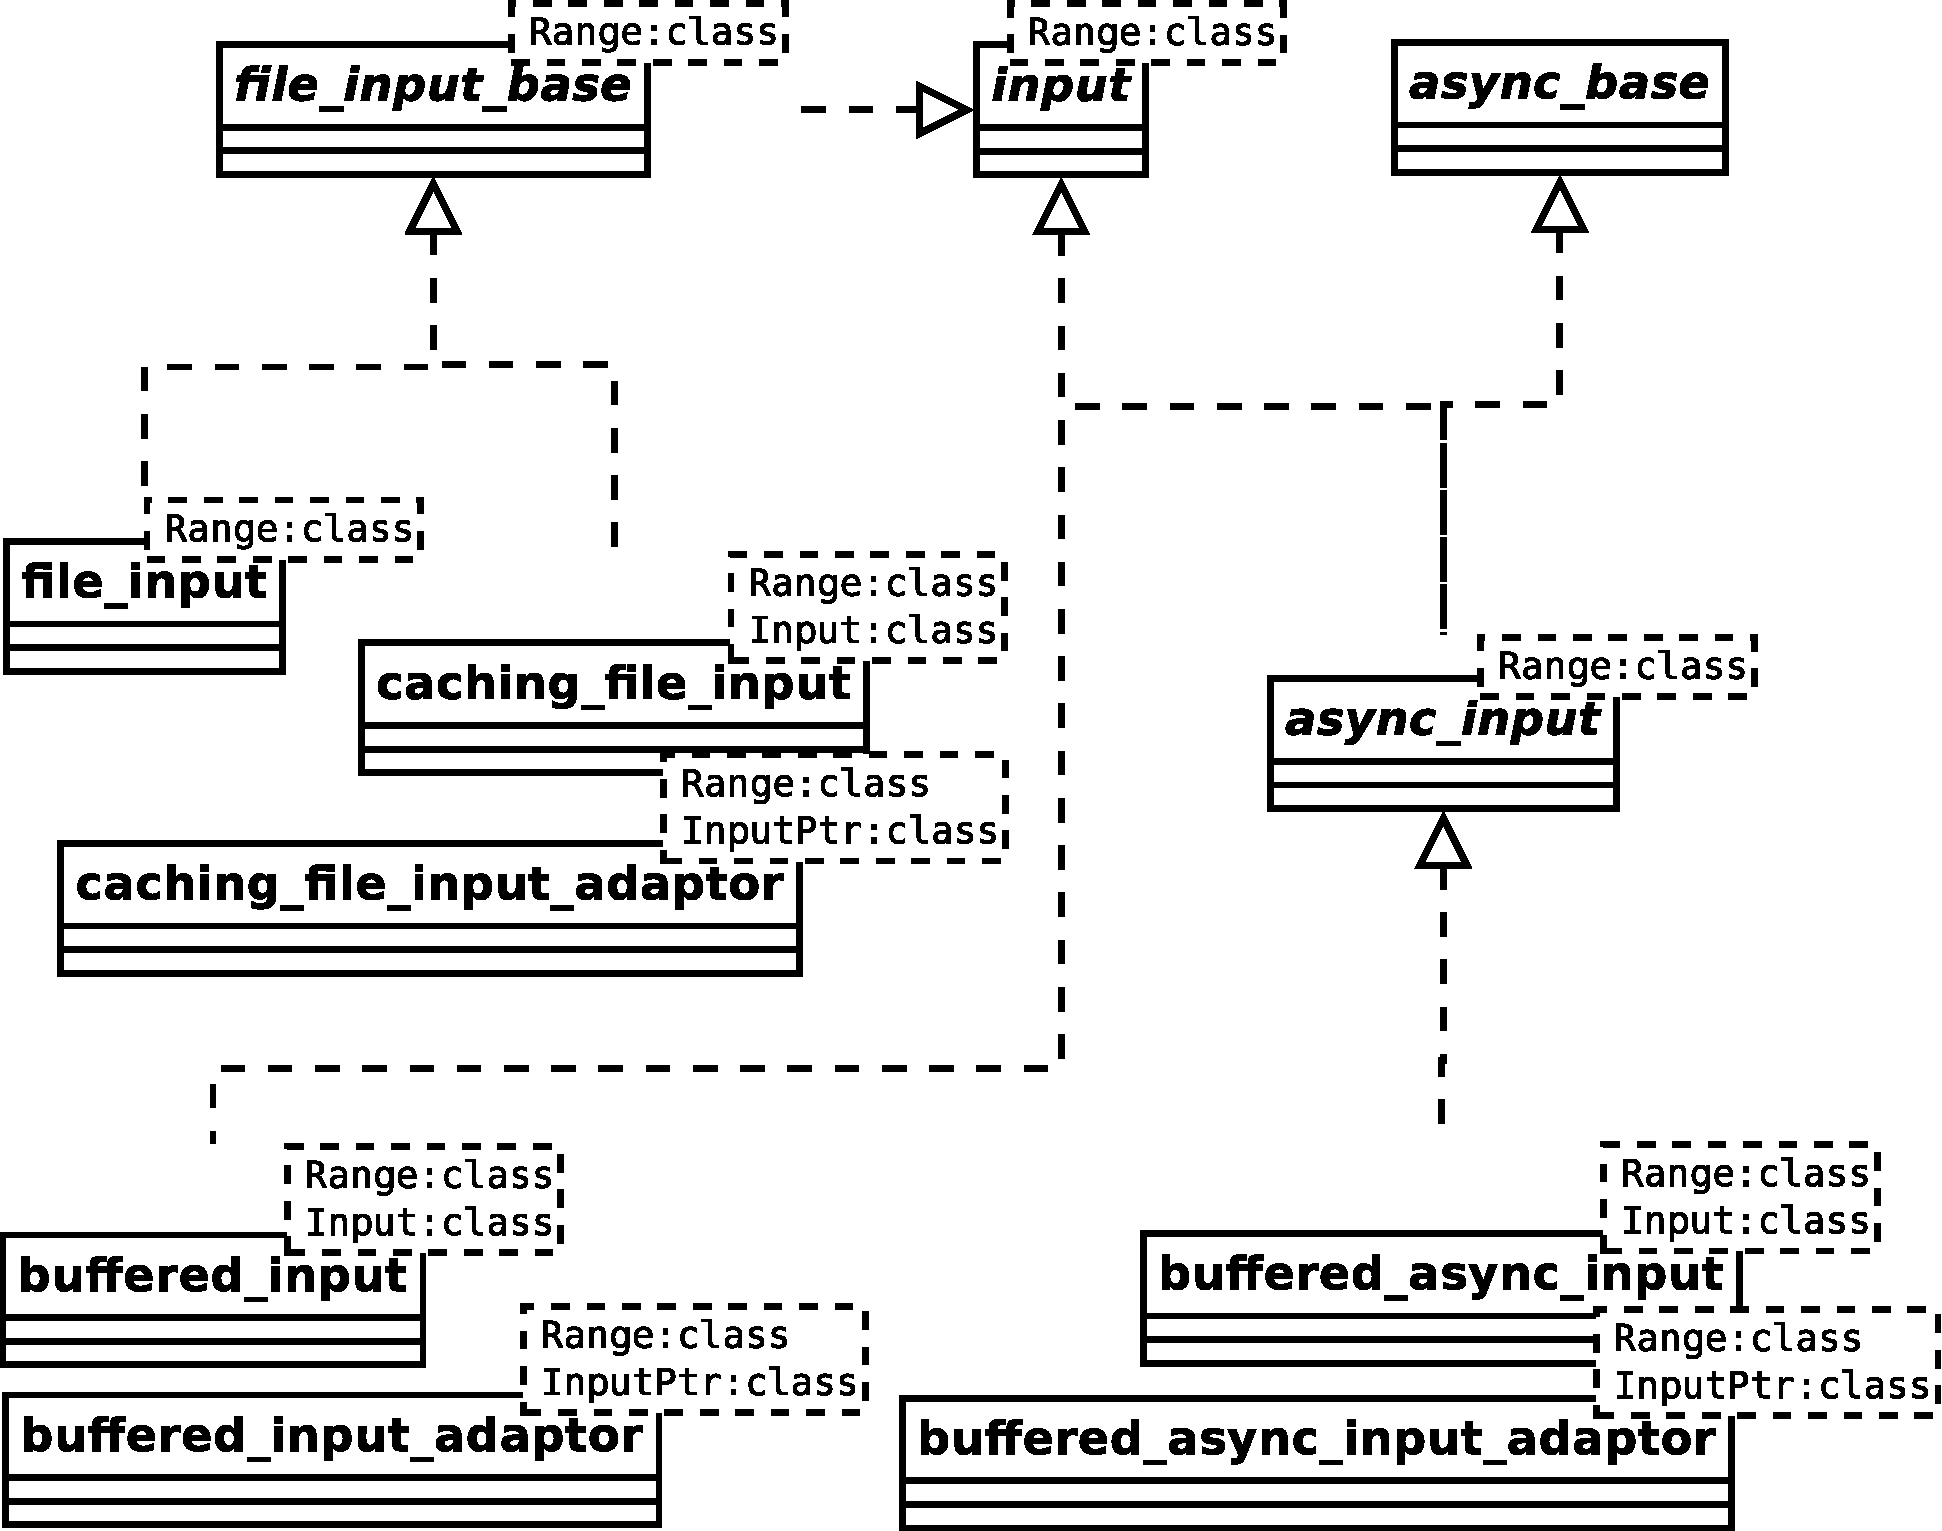
\includegraphics[width=\textwidth]{pic/io-class-input.pdf}
  \caption{UML class diagram of \type{psynth::io} input facilities.}
  \label{fig:inputuml}
\end{figure}

\begin{figure}[h]
  \centering
  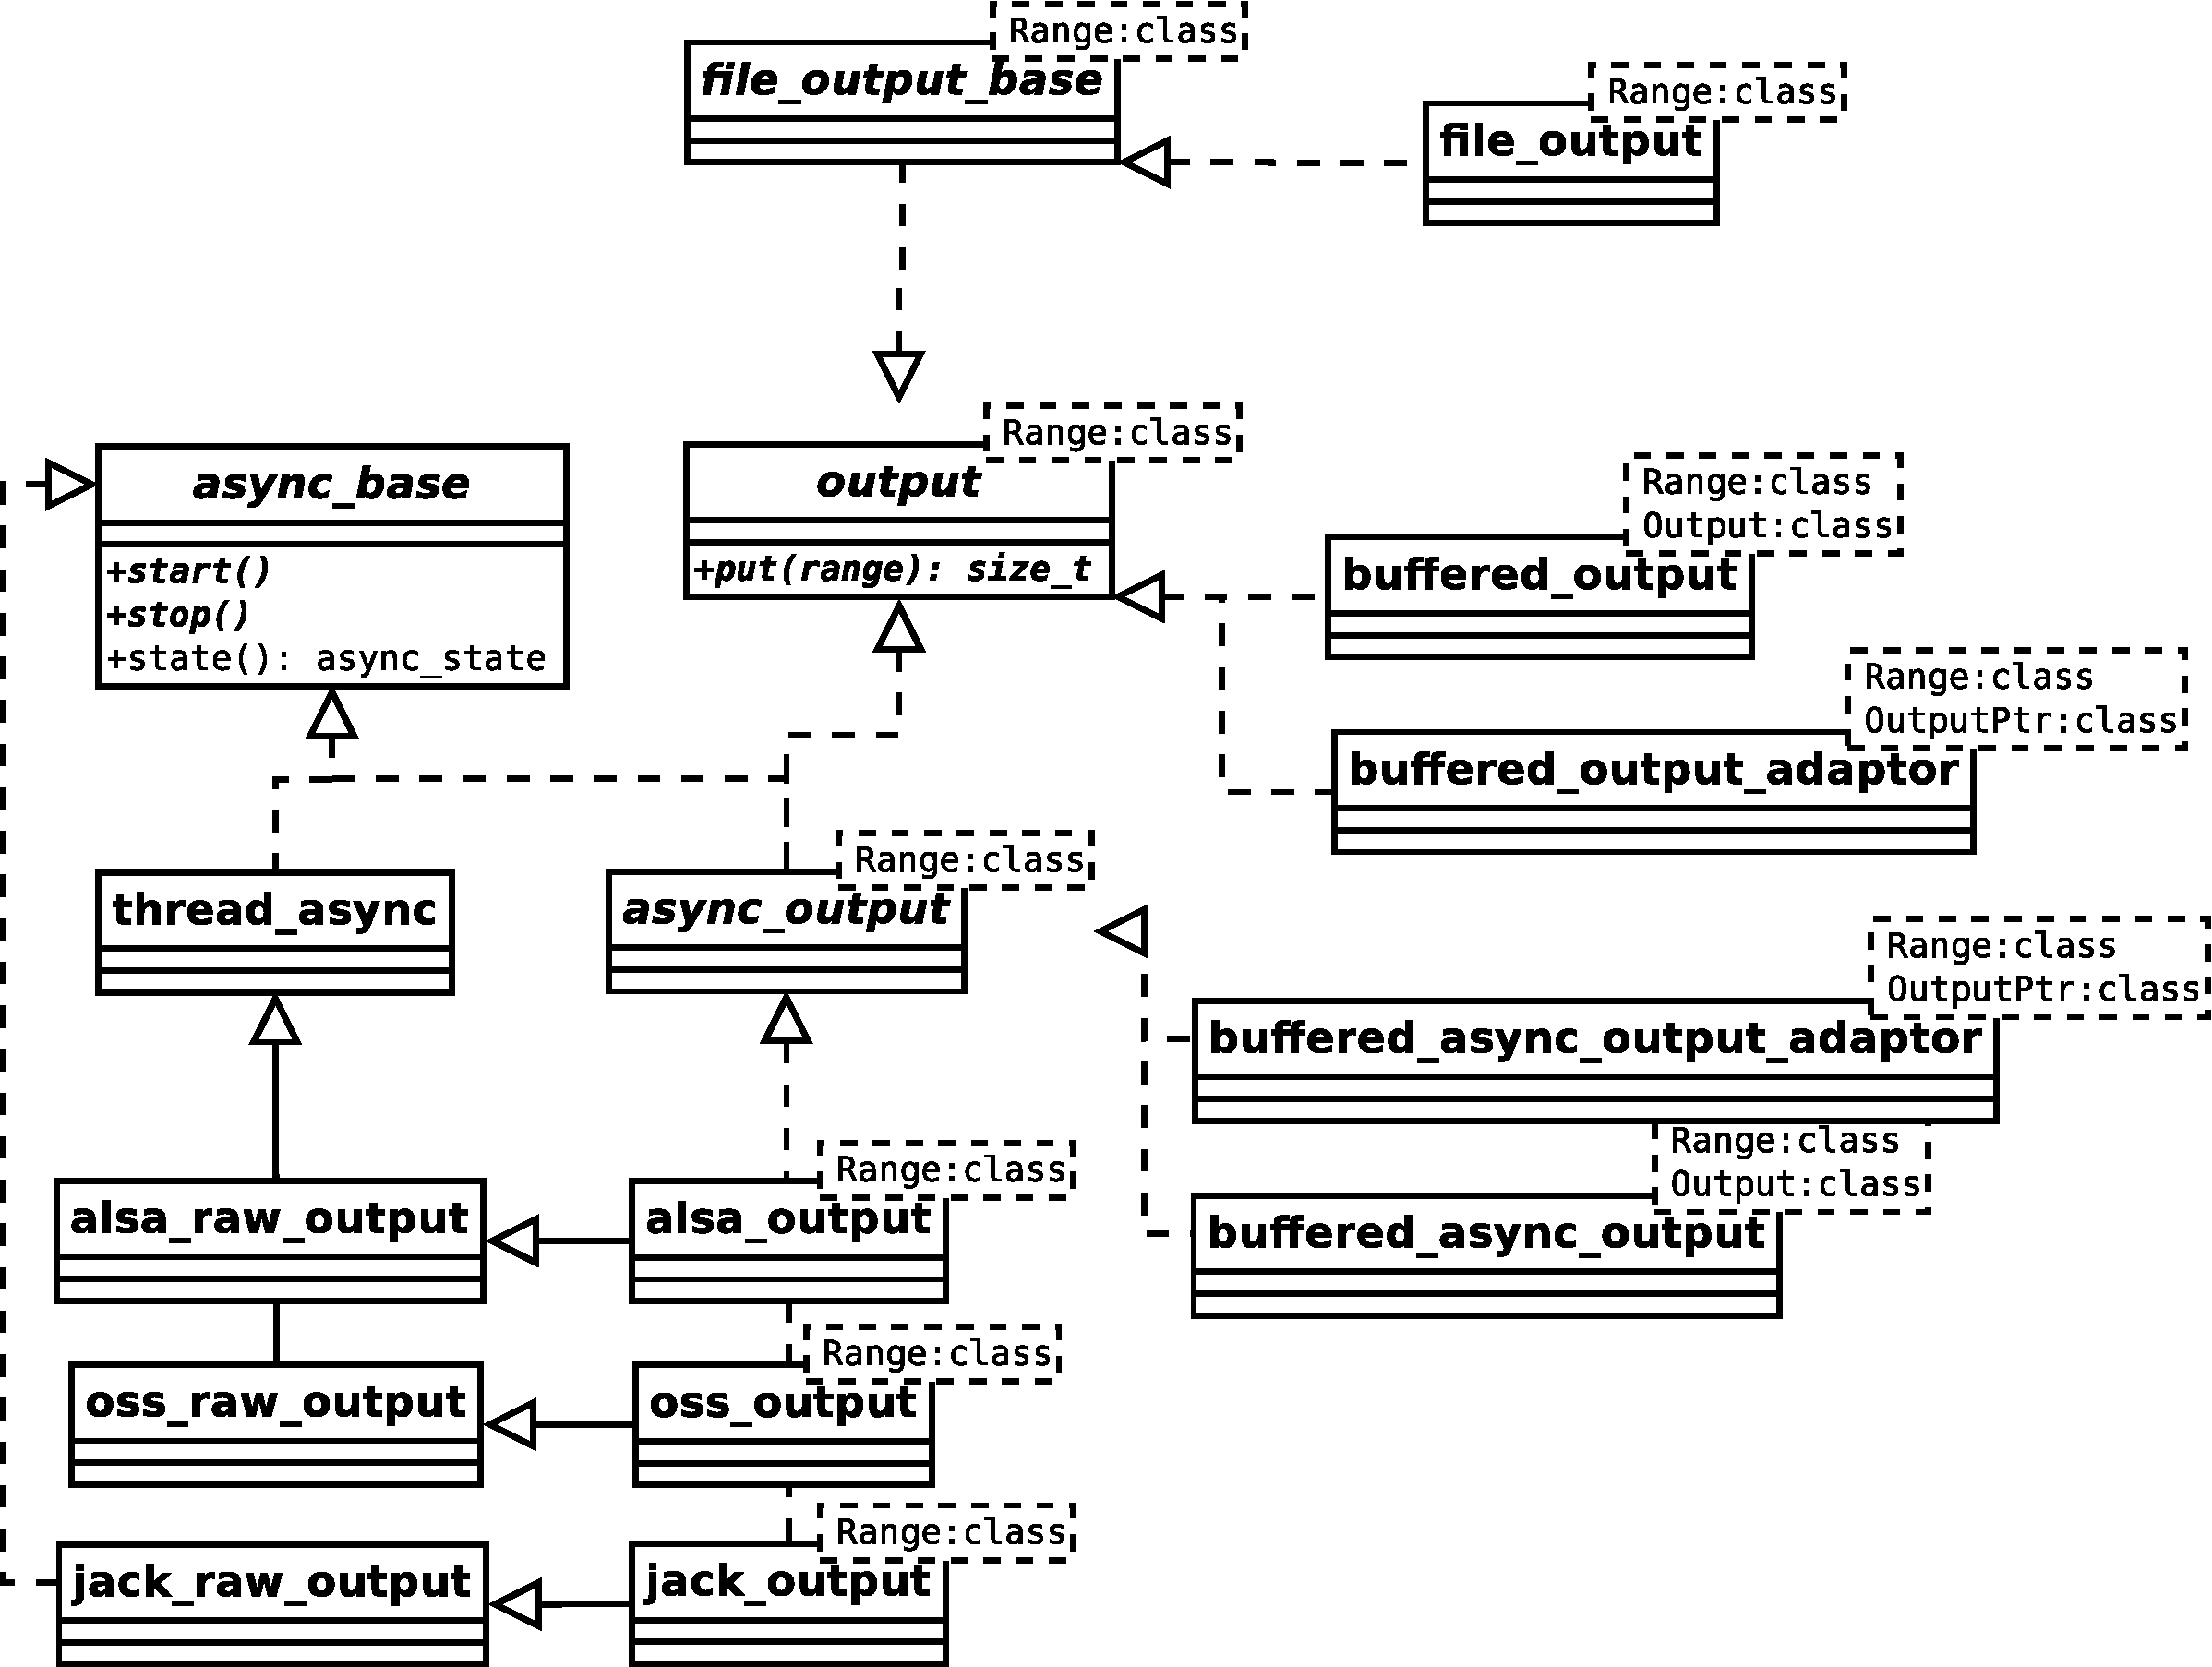
\includegraphics[width=\textwidth]{pic/io-class-output.pdf}
  \caption{UML class diagram of \type{psynth::io} output facilities.}
  \label{fig:outputuml}
\end{figure}

When talking about input and output, runtime polymorphism is more
important than static generality. We have to map the previous
facilities with the data that is out there in formats not always known
beforehand and provided by devices and interfaces whose availability
depend from one user system to another. Object orientation comes back
into play.

Figures \ref{fig:inputuml} and \ref{fig:outputuml} show the class
diagrams for the input and output parts of the module. We use the
Unified Modelling Language notation \cite{umlspec}. The doted boxes over
the corner of some classes list the formal parameter of generic
entities, an extension that was introduced in the 2.3 version of
UML. 

One should start reading the diagrams from the \type{input} and
\type{output} classes. They are the basic interfaces on which we build
the system. They are very simple, providing just a \type{take(const
  range\&)} and \type{put (const range\&)} abstract method
respectively --- and a typedef for accessing the actual argument for
its \type{Range} parameter. Because virtual functions can not be
templates themselves, these classes, when instantiated, provide
through those methods a hook for polymorphically sending or receiving
data to and from the external systems \emph{in only one
  format}. The next section shows how to work around this. Note also
that not every device support every format. Sometimes this is known
only at runtime --- and an exception will be thrown if trying to open
it in the wrong format --- but sometimes it can be known at compile
time (e.g., the OSS interface itself can not output planar data) 

Note that none of our I/O devices support \emph{open} and \emph{close}
functions. After our experience in previous versions of Psychosynth,
we have decided to simplify the interface and force specialisations to
use RAII --- opening the resource occurs in the constructor and closing it
in the destructor. This makes life easier to implementer of
specialisations (who are released from having to implement a state
machine) and for users of the library (who can be sure that a living
object is ready to use). If the same variable is to be used for
opening several files, one can use \type{swap} or the \emph{move
  constructor}. If the lifetime of variable does not match the one of
the resource \type{boost::optional} or a smart pointer should be used.

\subsubsection{Buffering}

For the reader who paid attention to our discussion on dynamic buffers
and ranges in section \ref{sec:ns-sound-beg} it might seem that
constraint of having to interface with only one type can be easily
solved by instantiating the I/O devices with a dynamic range. However,
in most cases that is not possible, because the device is opened to be
used in one mode of operation only and it will not be able to change
it until it is reopened. The most sensible solution is to use an
intermediate buffer where we convert the data before sending it or
receiving it. In order to avoid overhead due to buffering when
unneeded this behaviour is not provided by default.

The \type{buffered\_*} family of classes are adaptors that match from
a I/O interface in one format to another desired format. Because of
buffering, the target interface can be have a \texttt{dynamic\_range}
as parameter. The \type{buffered\_*\_adapter} types \emph{aggregate}
the adaptee via a pointer or smart pointer such that an already living
device can be adapted, or the buffer can be reused for several
devices. The other types \emph{compose} the adaptee managing their
lifetime --- the constructor parameters are forwarded from the
buffered adaptor constructor.

In order to convert among formats, this uses the
\emph{sound::co\-py\_and\_con\-vert\_fra\-mes} function that we
described earlier. This allows the user to provide a custom conversion
functor to convert among very specific formats.

\subsubsection{Asynchronous operation}
\label{sec:asyncio}

When data is to be provided in real time to or from a sound card,
chunks of audio data are to be processed as requested by the
device. All the descendants of \type{async\_base} are of this
kind. That interface provides \type{start ()} and \type{stop ()}
methods for controlling the state of the asynchronous
operation, plus others for checking its current status.

Whenever new data is sent or required by the device, a user specified
callback is executed with the number of frames as parameter, which
should in turn call \type{put ()} or \type{take ()} once the data is
ready or it can consume new information. Unless otherwise specified by
an specialisation, we assume that these functions can only be called
from the asynchronous callback. Also, we shall assume that the
callback is running under real time conditions, and thus it is
expected to have a time $O(n)$, where $n$ is the number of requested
samples, not block, perform no system calls and allocate no dynamic
memory.

The \type{thread\_async} class uses a thread to provide this kind of
asynchronous operation by and delegates the actual iteration inside an
infinite loop to the derived classes. Optionally, this class will try
to get real-time priority if requested\footnote{The \type{std::thread}
  standard class does not support priority changing. We use its
  \type{native\_handle} hook to request the new priority when POSIX
  threads is the underlying implementation. At this moment, we do not
  support real-time priority on other platforms.}. We do actually
request real-time priority in all the I/O devices based on the
\type{thread\_async} class.


\subsubsection{Raw I/O}

Most device management code does not depend on the audio format type,
and unnecessary object code bloat would be produced if it where in the
templates over the buffer range type. It is then abstracted in the
``raw'' I/O classes --- named after the pattern
\type{*\_raw\_\{input|output\}}. They can perform the I/O in an type
unsafe manner with incoming data in a void pointer. They are mostly an
implementation detail, but some users might find them handy as a
lightweight RAII wrapper over the underlying C interface.

\subsubsection{Caching input}

As we have noted, system calls should be avoided in the audio
processing thread. However, files should be read from disk, and
potentially decoded from hard formats, in order to play pre-recorded
samples or mix full songs. The \texttt{caching\_file\_input} family of
adaptors allow this kind of operation by reading the data in big
chunks on a separate thread. Because it has to do buffering anyway, it
can be used as an interface adaptor from one kind of buffer range to
another too, avoiding to use a worthless \texttt{buffered\_*\_output}
adaptor.

Our current implementation uses mutexes and condition variables, which
should be avoided, as we will deeply discuss in the next chapter. It
is planned to fix this in the future, section \ref{sec:fixringbuffer}
further discusses several solutions to this issue. Also, its
implementation is designed to aid writing \emph{samplers}. It has
interesting benefits, such as allowing to read the file
backwards. Also, when the change from forward to backwards reading is
made, the front and back pointers of its ring buffer are flipped and
the direction of reading and writing is reversed, such that the data
that was already loaded in those big chunk pre-fetchs can be reused.

\subsection{Synthesis module}
\label{sec:ns-synth}

In the \type{psynth::synth} namespace there is a whole bunch of
algorithms for sound synthesis, including oscillators, wave tables,
filters of all sorts, time stretchers, etc. Most of them are objects
that just provide an \texttt{update (...)} method taking buffer ranges
as needed plus several manipulators for their parameters.

We feel that their interface can be extensively improved, as
we discuss in section \ref{sec:fixsynth}. For this same reason, we
will avoid giving a detailed discussion of its design now.

\section{Validation}

\subsection{Unit testing}
\label{sec:sound-unittest}
unit testing serves to ensure that the actual behaviour of a function
matches its documented requirements. In this code it is very important
because: (1) because it is a library to be used by third party
developers, the proper functioning of every single method is as
important as the observable behaviour of the final application that we
may deploy alongside; and (2) because of the duck typing in template
metaprograms we need to ensure that all ``instantiation paths'' ---
i.e. code paths of the metaprogram --- compile without errors and lead
to correct execution.

The modules described in this chapter are evaluated with
a total 223 unit tests. All of them pass with a total of 1478
successful assertions. Note \ref{note:gistests} includes a more
detailed summary of the test suites involving these modules. Not all of
those unit tests have been written manually. Using
\type{BOOST\_UNIT\_TEST\_TEMPLATE} once can define a parametrised over
a type and that is later instantiated for every type in a given MPL
sequence. For example, we can compute the product of a MPL sequence of
buffer types with a metafunction and pass the result to the templated
unit test that checks proper conversion among buffer types,
simplifying a lot the amount of testing code --- avoiding
combinatorial explosion of code to test all instantiation paths.

\begin{mynote}[\texttt{psynth::sound} and \texttt{psynth::io} unit
  tests]
\label{note:gistests}
The user can run the unit tests by herself by running \texttt{make
  check} or running the \texttt{psynth\_unit\_tests} in the
\texttt{src/test} folder.  This kind of report may be generated
passing the \verb|--report=detailed| parameter when running the test
script directly.  {\small
\begin{verbatim}
Test suite "io_input_test_suite" passed with:
  177 assertions out of 177 passed
  110 test cases out of 110 passed

Test suite "io_output_test_suite" passed with:
  140 assertions out of 140 passed
  81 test cases out of 81 passed

Test suite "sound_ring_test" passed with:
  10 assertions out of 10 passed
  4 test cases out of 4 passed

Test suite "frame_iterator_test_suite" passed with:
  5 assertions out of 5 passed
  2 test cases out of 2 passed

Test suite "sound_peformance_test_suite" passed 
with:
  38 assertions out of 38 passed
  4 test cases out of 4 passed

Test suite "buffer_test_suite" passed with:
  14 assertions out of 14 passed
  2 test cases out of 2 passed

Test suite "sound_frame_test_suite" passed with:
  81 assertions out of 81 passed
  4 test cases out of 4 passed

Test suite "sound_sample_test_suite" passed with:
  1073 assertions out of 1073 passed
  14 test cases out of 14 passed
\end{verbatim}
}
\end{mynote}

\subsection{Performance}
\label{sec:sound-performance}

We claimed that static polymorphism and optimal algorithm selection
via template metaprogramming allow genericity with no overhead over
non-generic implementations. Given the performance constraints on the
real time audio processing thread, satisfying this property is a must.

To ensure that there is no overhead, we include a test suite that
compares the efficiency of the generic algorithm building blocks
provided by the library with hand-rolled loops performing the same
function. Listing \ref{lst:perf-gen} shows an example of such generic
function that you can compare with its concrete implementation in
\ref{lst:perf-nongen}. Note that for simplicity and because it does
not affect the results the non generic version is still parametrised
over the sample type $T$. One can read the whole performance test
suite in \texttt{src/test/psynth/sound/performance.cpp}.

\begin{lstlisting}[float=h,
  caption={Generic \texttt{for\_each} that asigns $(0,1)$ to every
  frame over non interleaved data},
  label=lst:perf-gen]
for_each_frame (_v, [] (F& f) { 
    f = F {0, 1};
});
\end{lstlisting}

\begin{lstlisting}[float=h,
  caption={Non generic \texttt{for\_each} that asigns $(0,1)$ to every
  frame over non interleaved data},
  label=lst:perf-nongen]
T* first = (T*)_v.begin ();
T* last  = first + _v.size () * 2;
while (first != last) {
    first [0] =  0;
    first [1] =  1;
    first     += 2;
}
\end{lstlisting}

We check the performance on some different cases that try to stress
different potential overhead corners, like using a different layout
from the natural order in the channel space, planar and interleaved
buffers, etc. Each test case test a kind of loop over a buffer of a
certain size. We test sizes of 32 and 4092 samples, as those are the
common bounds of buffer sizes used in audio (the lower the buffer
size, the better ---lower--- latency). This way we ensure that both
the per buffer and per sample overhead is minimal. Each test is
repeated $2^{21}$ times for buffers with 4096 samples, and $2^{26}$
times for buffers of 32 samples.

\begin{table}[h!]
  \centering\small
  \begin{tabular}{rl}
    Name & Meaning \\ \hline
    \type{s8b} & Interleaved stereo buffer with 8 bit samples.\\
    \type{rs8b} & Interleaved reversed stereo buffer with 8 bit samples.\\
    \type{s8pb} & Planar stereo buffer with 8 bit samples.\\
    \type{s8f} & Stereo frame with 8 bit samples.\\
    \type{rs8f} & Reversed stereo frame with 8 bit samples.\\
  \end{tabular}
  \caption{Acronyms for the parameter types in performance test result
    tables.}
  \label{tab:perfacrn}
\end{table}

We ran the tests in a Intel i5 M460 with four 2.53FHz cores. We
compiled tested the code with different versions of GCC compiled with
options \texttt{-O3 -std=c++0x}. Tables \ref{tab:perf4096} and
\ref{tab:perf32} show the results for GCC 4.5.2 with 4096 and 32
buffer size respectively and \ref{tab:perf4096-46} and
\ref{tab:perf32-46} show the results for GCC 4.6.0. The acronyms for
the concrete parameter types are expanded in table
\ref{tab:perfacrn}. All the timings are represented in $milliseconds$
computed as the mean of all iterations. The ``gain'' is defined as:
\begin{equation}
  Gain=\frac{T_{non\_psynth}}{T_{psynth}}  
\end{equation}
Such that a value greater than one signifies that the generic version
is faster and a value smaller than one implies that there is some
overhead.

The tables show interesting results. With GCC 4.5 the generic versions
performs as efficiently or better most of the time for larger buffer
sizes, however, there seems to be an additive constant that makes the
hand coded version slightly better when the buffer size is very
small. Surprisingly, GCC 4.6 changes this tendency and the generic
version actually gets more favourable results with short buffer
sizes. Actually the results are more even with this compiler in a
probable tendency in making optimisation techniques more general ---
i.e. dependent on the actual semantics of the code and not on
how you express it --- which is very desirable for generic code.

In any case, these results supports our claims that the performance
overhead, if any, is negligible. Sometimes the generic code is even
more efficient than a carefully hand-coded algorithm for a specific
audio format. The results also show that as soon as you add arithmetic
computations like in the \texttt{transform} test micro-optimisation in
the looping constructs is futile. Maybe testing with a wider variety
of compilers should be done, but that is not possible because few
support C++0x. Anyway, it is to expect that a compiler supporting
C++0x also has a decent optimiser and the we would get similar
results. Comparison of the generated object code would can be another
interesting mechanism for assuring the lack of overhead due to
generality. We did informal tests confirming our hypotheses that can
be repeated by the reader. Also, there are some similar object code
comparisons in the Boost.GIL video tutorial\footnote{Boost.GIL
  presentation:
  \url{http://stlab.adobe.com/gil/presentation/index.htm}} that the
interested reader can check --- given the similarities in GIL and
\texttt{psynth::sound} we can expect equivalent results.

We can safely state that the library passes the performance
requirements.

\begin{table}[p]
  \centering\small
  \begin{tabular}{c|c|c|c|c|c}
    Algo. & \multicolumn{2}{c|}{Parameters} & Psynth & Non-Psynth & Gain \\ \hline\hline

    %% fill_frames
    \multirow{4}{*}{\type{fill}} & \multirow{2}{*}{\type{s8b}} & \type{s8f} & 0.38147 & 0.38147 & 1 \\ 
    &  & \type{rs8f} & 0.376701 & 0.38147 & 1.0127 \\
    & \multirow{2}{*}{\type{s8pb}} & \type{s8f} & 0.195503 & 0.190735 & 0.9756 \\
    &  & \type{rs8f} & 0.190735 & 0.190735 & 1 \\ \hline

    %% for_each_frame
    \multirow{2}{*}{\type{for\_each}} & \multicolumn{2}{c|}{\type{s8b}} & 0.371933 & 0.376701 & 1.0128 \\
    & \multicolumn{2}{c|}{\type{s8pb}} & 0.286102 & 0.281334 & 0.9833 \\ \hline
    
    %% copy_frames
    \multirow{5}{*}{\type{copy}} & \multirow{3}{*}{\type{s8b}} & \type{s8b} & 0.38147 & 0.38147 & 1 \\ 
    &  & \type{rs8b} & 1.00136 & 1.05381 & 1.0524 \\ 
    &  & \type{s8pb} & 0.753403 & 0.753403 & 1 \\ 
    & \multirow{2}{*}{\type{s8pb}} & \type{s8pb} & 0.748634 & 0.762939 & 1.0191 \\ 
    &  & \type{s8b} & 0.38147 & 0.38147 & 1 \\ \hline

    %% transform_frames
    \multirow{4}{*}{\type{transform}} & \multirow{2}{*}{\type{s8b}} & \type{s8b} & 23.4795 & 23.4842 & 1.0002 \\ 
    &  & \type{s8pb} & 23.4842 & 23.4842 & 1 \\
    & \multirow{2}{*}{\type{s8pb}} & \type{s8b} & 23.4842 & 23.4842 & 1 \\
    &  & \type{s8pb} & 23.4842 & 23.4842 & 1 \\ \hline
  \end{tabular}
  \caption{Performance tests  4096 buffer size with GCC 4.5.}
  \label{tab:perf4096}
\end{table}

\begin{table}[p]
  \centering\small
  \begin{tabular}{c|c|c|c|c|c}
    Algo. & \multicolumn{2}{c|}{Parameters} & Psynth & Non-Psynth & Gain \\ \hline\hline

    %% fill_frames
    \multirow{4}{*}{\type{fill}} & \multirow{2}{*}{\type{s8b}} & \type{s8f} & 0.0103563 & 0.0104308 & 1.0071 \\ 
    &  & \type{rs8f} & 0.0103563 & 0.0104308 & 1.0071 \\
    & \multirow{2}{*}{\type{s8pb}} & \type{s8f} & 0.0125915 & 0.0104308 & 0.8284 \\
    &  & \type{rs8f} & 0.018999 & 0.0139326 & 0.7333 \\ \hline

    %% for_each_frame
    \multirow{2}{*}{\type{for\_each}} & \multicolumn{2}{c|}{\type{s8b}} & 0.00149012 & 0.00141561 & 0.9499 \\
    & \multicolumn{2}{c|}{\type{s8pb}} & 0.0090152 & 0.0064075 & 0.7107 \\ \hline

    %% copy_frames
    \multirow{5}{*}{\type{copy}} & \multirow{3}{*}{\type{s8b}} & \type{s8b} & 0.012517 & 0.012219 & 0.9761 \\ 
    &  & \type{rs8b} & 0.0112504 & 0.0108033 & 0.9602 \\ 
    &  & \type{s8pb} & 0.0179559 & 0.0175089 & 0.9751 \\ 
    & \multirow{2}{*}{\type{s8pb}} & \type{s8pb} & 0.0239909 & 0.0243634 & 1.0155 \\ 
    &  & \type{s8b} & 0.0136346 &  0.00394881 & 0.2896 \\ \hline

    %% transform_frames
    \multirow{4}{*}{\type{transform}} & \multirow{2}{*}{\type{s8b}} & \type{s8b} & 0.183433 & 0.183508 & 1.0004 \\ 
    &  & \type{s8pb} & 0.183508 & 0.183433 & 0.9995\\
    & \multirow{2}{*}{\type{s8pb}} & \type{s8b} & 0.183433 & 0.183508 & 1.0004 \\
    &  & \type{s8pb} & 0.183508 & 0.183433 & 0.9995 \\ \hline
  \end{tabular}
  \caption{Performance tests for 32 buffer size with GCC 4.5.}
  \label{tab:perf32}
\end{table}

\begin{table}[p]
  \centering\small
  \begin{tabular}{c|c|c|c|c|c}
    Algo. & \multicolumn{2}{c|}{Parameters} & Psynth & Non-Psynth & Gain \\ \hline\hline

    %% fill_frames
    \multirow{4}{*}{\type{fill}} & \multirow{2}{*}{\type{s8b}} & \type{s8f} & 0.557899 & 0.562668 & 1.0085 \\ 
    &  & \type{rs8f} & 0.557899 & 0.557899 & 1 \\
    & \multirow{2}{*}{\type{s8pb}} & \type{s8f} & 0.190735 & 0.190735 & 1 \\
    &  & \type{rs8f} & 0.190735 & 0.185966 & 0.9749 \\ \hline

    %% for_each_frame
    \multirow{2}{*}{\type{for\_each}} & \multicolumn{2}{c|}{\type{s8b}} & 0.557899 & 0.562668 & 1.0085 \\
    & \multicolumn{2}{c|}{\type{s8pb}} & 0.276566 & 0.286102 & 1.0344 \\ \hline
    
    %% copy_frames
    \multirow{5}{*}{\type{copy}} & \multirow{3}{*}{\type{s8b}} & \type{s8b} & 0.739098 & 0.743866 & 1.0064 \\ 
    &  & \type{rs8b} & 1.05381 & 0.934601 & 0.8868 \\ 
    &  & \type{s8pb} & 0.753403 & 0.753403 & 1 \\ 
    & \multirow{2}{*}{\type{s8pb}} & \type{s8pb} & 0.867844 & 0.743866 & 0.8571 \\ 
    &  & \type{s8b} & 0.38147 & 0.386238 & 1.0125 \\ \hline

    %% transform_frames
    \multirow{4}{*}{\type{transform}} & \multirow{2}{*}{\type{s8b}} & \type{s8b} & 23.4842 & 23.4795 & 0.9997 \\ 
    &  & \type{s8pb} & 23.4842 & 23.4842 & 1 \\
    & \multirow{2}{*}{\type{s8pb}} & \type{s8b} & 23.4842 & 23.4842 & 1 \\
    &  & \type{s8pb} & 23.4842 & 23.4795 & 0.9997 \\ \hline
  \end{tabular}
  \caption{Performance tests for 4096 samples with GCC~4.6.}
  \label{tab:perf4096-46}
\end{table}

\begin{table}[p]
  \centering\small
  \begin{tabular}{c|c|c|c|c|c}
    Algo. & \multicolumn{2}{c|}{Parameters} & Psynth & Non-Psynth & Gain \\ \hline\hline

    %% fill_frames
    \multirow{4}{*}{\type{fill}} & \multirow{2}{*}{\type{s8b}} & \type{s8f} & 0.00625849 & 0.00625849 & 1 \\ 
    &  & \type{rs8f} & 0.00499189 & 0.00499189 & 1 \\
    & \multirow{2}{*}{\type{s8pb}} & \type{s8f} & 0.0103563 & 0.0104308 & 1.0071 \\
    &  & \type{rs8f} & 0.0104308 & 0.0104308 & 1 \\ \hline

    %% for_each_frame
    \multirow{2}{*}{\type{for\_each}} & \multicolumn{2}{c|}{\type{s8b}} & 0.00618398 & 0.00625849 & 1.0120 \\
    & \multicolumn{2}{c|}{\type{s8pb}} & 0.0064075 & 0.0064075 & 1 \\ \hline

    %% copy_frames
    \multirow{5}{*}{\type{copy}} & \multirow{3}{*}{\type{s8b}} & \type{s8b} & 0.012219 & 0.0125915 & 1.0304 \\ 
    &  & \type{rs8b} & 0.00782311 & 0.0111014 & 1.419 \\ 
    &  & \type{s8pb} & 0.0169873 & 0.0172853 & 1.018 \\ 
    & \multirow{2}{*}{\type{s8pb}} & \type{s8pb} & 0.0243634 & 0.0219047 & 0.899 \\ 
    &  & \type{s8b} & 0.0114739 &  0.0160933 & 1.4026 \\ \hline

    %% transform_frames
    \multirow{4}{*}{\type{transform}} & \multirow{2}{*}{\type{s8b}} & \type{s8b} & 0.183433 & 0.183508 & 1.0004 \\ 
    &  & \type{s8pb} & 0.183433 & 0.183582 & 1.0004 \\
    & \multirow{2}{*}{\type{s8pb}} & \type{s8b} & 0.183433 & 0.183433 & 1 \\
    &  & \type{s8pb} & 0.183433 & 0.183508 & 1.0004 \\ \hline
  \end{tabular}
  \caption{Performance tests for 32 buffer size with GCC 4.6.}
  \label{tab:perf32-46}
\end{table}

\subsection{Integration and deployment}

The module was first developed separately from the main development
branch in a branch called \texttt{gil-import}. Once the previous tests
were passed, the former signal representation classes and I/O code was
removed from the code base. The upper layers --- mainly the
\texttt{graph} layer --- was adapted to use the new library. Note
that, given that we will mostly rewrite the \texttt{graph} layer in
the next iteration we tried to make minimal changes to get the project
compile and run properly again.

The system was then \emph{peer reviewed} by project collaborators,
mainly by the maintainer of the Ubuntu/Trinux packages Aleksander
Morgado\footnote{Aleksander Morgado's web blog:
  \url{http://sigquit.wordpress.com}}. After minor bugfixing, we
agreed to make a new Psychosynth 0.2.0 release that included the new
code described in this chapter and some other fixes and modifications
developed alongside.

The official changelog briefing for this release is included in note
\ref{note:changelog02}.

\begin{mynote}[Changelog of Psychosynth 0.2.0]
\label{note:changelog02}
\begin{itemize}
\item New audio processing and I/O subsystem based on template programming
for generic yet efficient sound signals.

\item The extreme latency when using ALSA bug seems to be fixed in
  some cases.

\item No longer depend on libvorbis, libsndfile can now handle ogg and flac
files too.

\item No longer depend on \texttt{libsigc++}, using \texttt{boost::signals}
  which, which is a bit slower but neglibe and this simplifies the
  dependencies.

\item The mouse wheel now scrolls in the object selector.

\item The object selector no longer lets mouse clicks pass through.  

\item Backwards reproducing a sample works a bit better now too.

\item Some new niceties in the framework base layer, including some
  experiments on applying the C3 class linearisation algorithm in raw
  C++.

\item C++0x features are being used in the code. For GCC, this means
  version 4.5 shall be used. We doubt it will compile with any other
  compiler (maybe latest VS), but users are welcomed to try and report.

\item For this same reason, Boost.Threads is no longer a dependency,
  we use STL threads instead.
\end{itemize}
\end{mynote}

\section{Conclusions}

In this iteration we developed a generic approach to representation
and input and output of audio data. We do not have any records of
any audio software using such paradigm in their code, so this
development have been exploratory and has a lot of value in its
novelty. This however delayed our development more than expected in
our original plan.

\subsection{Benefits and caveats}
\label{sec:soundbenefits}

The three main advantages in the new code are:
\begin{enumerate}
\item Code can be mostly abstracted from the audio format
  representation while retaining near optimal performance. Because
  generality allowed decoupling orthogonal concepts, each audio
  representation factor can be optimised and tuned for computational
  accuracy on its own, leading to higher quality code with lower
  maintenance cost as we avoid the combinatorial explosion that
  happens otherwise.

\item Algorithms correctly written with our generic facilities have a
  performance equivalent to the hand-written code. When a certain
  algorithm has not general interpretation or can not be efficiently
  implemented generally, the library still allows for the algorithm to
  be written with for a concrete or a constrained family of audio
  formats.

\item Because the signal format is encoded in the data type, we can
  either statically check that the data is in the correct format
  through our processing chain, or trivially enforce runtime checks
  when the format is unknown at compile time (via
  \texttt{dynamic\_buffer} and similar tools), leading to more secure
  code.
\end{enumerate}

Also, because a lot of learning have happened since the old code base
was written, the new code is better written and quite safer, making
use of exceptions and scope guards \cite{alexandrescu00gener}.

Even though we believe the benefits outweight the drawbacks, we have
to acknowledge the caveats of our new approach, the most relevant
being:
\begin{enumerate}
\item The new code uses advanced C++ programming techniques that many
  programmers find hard to understand. Thus, it might be harder for
  casual contributors to join the project in the future.

\item In the absence of real language support for concepts, template
  metaprograms leak their implementation in user code's compilation
  errors. This is so because, actually, by expanding the type
  instantiations in the compilation error, the compiler is actually
  showing a full backtrace of the metaprogram. This leads to cryptic
  error messages that often obfuscate the real source of the problem,
  discouraging novel developers.

\item Template metaprograms take longer to compile. However, proper
  usage of the new \texttt{extern template} facility should avoid
  redundantly instantiating templates in different translation units
  only to be discarded by the linker mostly solving this issue. Also,
  because the compiler generates different object code for each audio
  format, thoughtless use of the library can lead to code bloat and
  too large binary size.
\end{enumerate}

\subsection{Future work}

While the current status of the library is quite satisfactory for our
needs, there is still a lot of room for improvement that we will
postpone since they fall outside this project's scope. Nonetheless it
is worth enumerating them:

\subsubsection{Lock free ring buffers}
\label{sec:fixringbuffer}

The audio processing thread has real time constraints. As we
introduced in note \ref{note:realtime} this implies, among other
things, forbidding the usage of mutexes. However, our ring buffers
have not been tested for thread safety and mutexes should be used when
shared among different threads. This happens in our
\texttt{caching\_file\_input} implementation. The problem is specially
severe when the audio processing thread is running with higher
priority, because \emph{priority inversion} occurs
\cite{kim03basic}. While our current Alsa and OSS output systems do
not attempt rising their thread priority, the Jackd subsystem executes
the audio processing callback in a real-time mode thread and thus the
problem can become significant.

Locking is done with care and in practice we have experience no buffer
underruns due to this problem, even with high number of caching file
readers in execution.  However, for correctness and better support of
Jackd, we should implement a lock-free ring buffer
\cite{valois94lock, michael95correction} that does not require
using special synchronisation. Jackd actually provides a C
implementation that can serve as a basis for ours. The most important
interface change is that only one reader should be permitted --- we
can embed the read pointer inside the data structure. Also, the
``backwards'' operation mode in our current implementation might
introduce an unexpected complexity in the implementation.

\subsubsection{Virtual and adapted iterators and ranges}
\label{sec:fixsynth}

Boost.GIL included a ``locator adapter'' and ``virtual locator''
notions that allowed creating or modifying images lazily via a
function object. We discarded implementing the virtual ones because
they were coupled to their \texttt{locator} concept which is specific
to the problem of image representation --- locators are in practice 2D
iterators. Moreover, they used the indexed position in the image as
the parameter to the function object that synthesised the
image. However, because audio is processed in chunks, the position in
the audio buffer is meaningless for the synthesis or filter function
--- instead, some stateful function object which includes a notion of
time position related to the frame rate is needed. Thus, many
unexplored design decisions should be taken, and the interactions with
other similar libraries like Boost.Iterator\footnote{The
  Boost.Iterator Library:
  \url{http://www.boost.org/doc/libs/release/libs/iterator}} and
Boost.Range\footnote{The Boost.Range Library:
  \url{http://www.boost.org/doc/libs/release/libs/range}} should be
carefully evaluated.

\subsubsection{Better arithmetic support}

The library includes some basic arithmetic support for samples. There
are few complications when developing full generic arithmetic support
for samples and frames. As Lubomir Bourdev, lead developer of
Boost.GIL, stated it in an email conversation with us:

\begin{quotation}
``Doing arithmetic operations is tricky for a number of reasons:

\begin{itemize}
\item What do you do on overflow? Clip, throw exception, allow out of
  range values?

\item What is the type to be used during conversion? Even if the
  source and destination have the same type, the operation might need
  to be done in another type and then cast back.

\item Certain arithmetic operations have no meaningful interpretation
  as far as color is concerned, such as multiplying one pixel by
  another. 
\end{itemize}

Because of issues like these we have not tackled the problem of
providing arithmetic operations, but we have provided generic
operations that can be done per channel or per pair of channels which
could be the basis for arithmetic operations.''
\end{quotation}

Nonetheless with time and effort the problem could be
approached making some compromises. Some of the issues Lubomir states
have different answers for sound processing, in fact, allowing out of
range values is the best answer for the first question given the fact
that sound amplitude is not naturally constrained and clipping is
introduced only by the DAC hardware or when moving from floating to a
fixed point representation. Maybe, not all those questions have to be
answered in order to improve the arithmetic support.

One of the main annoyances when writing a generic algorithm is using
the per sample \texttt{static\_*} algorithms. Using them we could
write a simple arithmetic layer for frames that would simplify the
user code. However, even though we do not have experimental data, we
believe this straightforward solution could introduce overhead. This
is because every \texttt{static\_*} unrolls one statement per
channel. Thus, a simple frame arithmetic expression would in fact
result into many sequence points that is yet to be tested whether
compilers can optimise properly.

This is not a dead end. Using the \emph{expressions templates}
\cite{veldhuizen95expression} technique and r-value references we can
perform transformations with the aid of metaprogramming such that
sequence points are not introduced by the arithmetic expression
itself. A expression template framework like Boost.Proto\footnote{The
  Boost Proto library:
  \url{http://www.boost.org/doc/libs/release/libs/proto}}
\cite{niebler07proto} could be of great help. Moreover, with careful
studying of the audio DSL's studied in section \ref{sec:dsl} and the
usage of these same techniques the scope of such effort could be
broadened to build a full sound synthesis and processing EDSL for
C++. Indeed, this would allow writing specific optimisations in this
arithmetic layer itself. It would be specially interesting to optimise
for usage of SIMD\footnote{Single Instruction Multiple Data. These
  instructions can operate on several arguments at the same time. They
  are very useful in multimedia applications. For example, all the
  samples in a multi-channel audio frame could be updated with one
  single instruction, multiplying the performance. The SSE family of
  multimedia extensions provided by Intel processors are is the most
  widespread set of SIMD instructions.} instructions of modern
processors. While this can be done now in a per-algorithm basis, doing
so in a frame-arithmetic layer would hide all this complexity to the
DSP developer providing a significant performance boost for free.

\subsubsection{Submission to Boost}

In our conversations with Lubomir Bourdev he suggested submitting our
library for inclusion in the Boost package. However, there are few
issues that we should tackle before that:

\begin{enumerate}
\item A lot of code is algorithmically identical to that of Boost.GIL
  with changes only in terminology. A lot of work in properly
  abstracting such common parts should be made to avoid code
  repetition and doubled maintenance effort inside Boost.

\item As we said earlier, interesting interactions can emerge with
  the Boost.Iterator and Boost.Range libraries. We believe that any
  possible issues and unneeded incompatibilities with those libraries
  should be solved before submission into Boost.

\item Boost is written in C++03 standard, while our code uses
  C++0x. Moreover, our code has dependencies with other submodules in
  \texttt{psynth::base}, specially the expection and logging
  system. While these dependencies are not too strong, the effort made
  to polish these corners is outside the scope of the current project.
\end{enumerate}

%%% Local Variables: 
%%% mode: latex
%%% TeX-master: "00-main"
%%% End: 
